\documentclass{thesis}

% TX Fonts を使う
\usepackage{txfonts}
\usepackage{url}
\usepackage{algorithm}
\usepackage{algorithmic}
\usepackage[dvipdfmx]{color}
\usepackage{multirow}
\usepackage{subfigure}
\usepackage{indentfirst}

\begin{document}

% 目次
\tableofcontents
%--ここから本文---
\chapter{序論}
%第1章 まえがき

%1章1節
\section{研究背景および目的・目標}
近年では,IoT(Internet of Things)の普及が進んでおり,様々なものがインターネットに繋がる時代である.インターネトに繋がるものをIoT機器(IoTデバイス)といい,例として家電や自動車・産業用ロボットなどが挙げられる.
IoTを実現する上で,周囲の情報を検知するセンシングデバイスやネットワークは必要不可欠である.
そして,センシングデバイスがインターネットに繋がることで,外部の悪意のある第三者からの攻撃により,データを盗聴・改ざんする恐れが懸念される.

第三者からの攻撃事例に,タイヤ空気圧監視システムへの攻撃事例がある\cite{maegaki}.
タイヤ空気圧監視システム(TPMS:(Tire Pressure Monitoring System))とは,
タイヤの空気圧を常時監視するシステムであり,空気圧が低いタイヤで高速走行をすることによるタイヤバースト事故を防ぐ効果が期待される.
しかし,このTPMSの無線通信には脆弱性があることが問題となっている.
その問題の一つとして,TPMSでは通信メッセージが暗号化されていないため,盗聴解析が容易になるという点がある.
また, TPMSの空気圧報告メッセージになりすますことができるという問題点もある.
この事例から,センシングデバイスにおいて,ネットワーク上の脆弱性があることで外部からの攻撃によるデータの盗聴・改ざんが行われてしまうリスクがあることから,セキュリティ対策が不可欠となることが分かる.

センシングデバイスのセキュリティ対策の一つに認証・暗号化がある.
しかしながら,AESなど従来の暗号化方式は処理負荷が高いことから処理性能の低いセンシングデバイスには導入困難であるため,現在市場に出回っているセンシングデバイスには認証・暗号化といったセキュリティ対策が不十分で,脆弱性があると考えられる.
そこで,センシングデバイスなど,処理性能の低いIoT機器において,
極めて小さい処理負荷で認証と暗号化通信のできる軽量なセキュリティ対策が求められる.

本研究では,処理能力の低いセンシングデバイスで構成されるIoTシステムにおいて,デバイスとエッジサーバー間の
安全なデータ通信を行うセキュアな組込みシステムを開発することを目的とする.
具体的には,高知工学科大学の清水明宏教授が処理能力の低い装置へのセキュリティ機能実装のために
開発されたワンタイムパスワード認証方式SAS-L2をIoTセンシングデバイス
に実装することで,デバイス間の相互認証およびセンシングデータの暗号化通信方法を実現する.
なお,本研究は,2人チーム(浅野美咲,内山田隆太)でV字開発モデルに従って処理能力の低いセンシングデバイスで構成されるSAS-L2認証を導入したセキュアなIoTシステムの開発を行う.
システムの設計にはUMLを利用する.
チームメンバーの2人で分担し,内山田がエッジサーバーの実装,浅野がエッジデバイスの実装を行う.




%1章2節

\section{本論文の構成}
本論文の構成は以下の通りである.
第1章では,研究の背景および目的・目標について述べる.
第2章では,本論文に必要な暗号化手法と通信プロトコル,システム開発プロセスに関する用語について述べる.
第3章では,SAS-L2認証について述べる.
第4章では,センシングデータ通信の暗号化について述べる.
第5章では,開発したシステムの概要について述べる.
第6章では,システムの設計・テスト項目について述べる.
第7章では,実装したシステムの検証結果と考察を述べる.
第8章では,本論文のまとめを述べる.


\chapter{準備}
%第2章:定義

本章では,本論文で必要な暗号化手法と通信プロトコル,システム開発プロセスに関する用語について説明する.
\section{暗号化手法}
本節では,従来の暗号化方式としてAESとバーナム暗号について説明する.
%2章1節
\subsection{AES(Advanced Encryption Standard)}
AESとは,無線LANなどの通信データの暗号化に用いられる暗号化アルゴリズムの一つである.
AESは,共通鍵暗号方式であり,同じ暗号鍵を利用してデータの送信者が暗号化,データの受信者が
復号化を行う.また,128・192・256bitのいずれかの鍵長を使用することが可能である.
AESアルゴリズムは,以下の4種類の変換を順番に用いる\cite{AES}.
\begin{description}
	\item[SubBytes] 16バイトごとに区切ったデータに対し,テーブルを用いて1バイト単位
で置換する.
	\item[ShiftRows] 1バイト単位でデータの順序を入れ替える.
	\item[MixColumns] 4バイトごとに行列演算を行う.
	\item[AddRoundKey] 128・192・256bitのいずれかの暗号鍵を基に生成した鍵で変換する.
\end{description}
この一連処理を複数回繰り返し暗号化を行う.
復号化では,以上の4種類の変換と逆の変換を行う.
\subsection{バーナム暗号}
バーナム暗号とは,1917年にギルバート・バーナムが発明した暗号化方式である\cite{banamu}.
1949年にはシャノンによって,理論的に解読不可能であることが証明されている.
バーナム暗号は暗号化と復号化の際に同じ秘密鍵を使用する共通鍵暗号方式であり,
秘密鍵は一度しか使用できないという特徴がある.秘密鍵が一度しか使用できなことから,
暗号化と復号化を行う度に,秘密鍵を共有し直さなければならない.

%2章2節
\section{通信プロトコル}
本節では,本研究で用いた通信プロトコルであるTCPとUDPについて説明する.
\subsection{TCP(Transmission Control Protocol)}
TCPとは,データの送信を開始する前に,送信ホストと受信ホストの間で回線の接続をするコネクション型で,信頼性のあるトランスポート層のプロトコルである\cite{tcp/udp}.両端のホスト間でデータの到達性を保障する.ネットワークの帯域幅を有効に利用する仕組みや,ネットワークの混雑を和らげる仕組みなど,様々な機能が組み込まれており信頼性の向上が図られる.
%2章3節
\subsection{UDP(User Datagram Protocol)}
UDPとは,TCPと異なりコネクションの確立や切断処理がないコネクションレス型で,信頼性のないトランスポート層プロトコルである\cite{tcp/udp}.また,UDPには送信されるデータの誤りや順序の違いなどを検出する機能がない.パケット数が少ない通信や,ビデオ音声などのマルチメディア通信に向いている.

%2章5節
\section{システム開発プロセス}
本節では,本研究でのシステム開発のプロセスに関する用語について説明する.
\subsection{V字開発モデル}
V字開発モデルとは,テストを重視し,図\ref{fig:vmodel}の様に左側の要件定義や設計のプロセスと対応させる.
例えば,図\ref{fig:vmodel}では詳細設計には単体テストが配置されている.
これは,詳細設計の正しさを単体テストによって確認し,
単体テストで不具合が見つかった場合は,左側の対応するプロセスである詳細設計に戻って修正する\cite{vmodel}.

\begin{figure}[H]
\begin{center}
	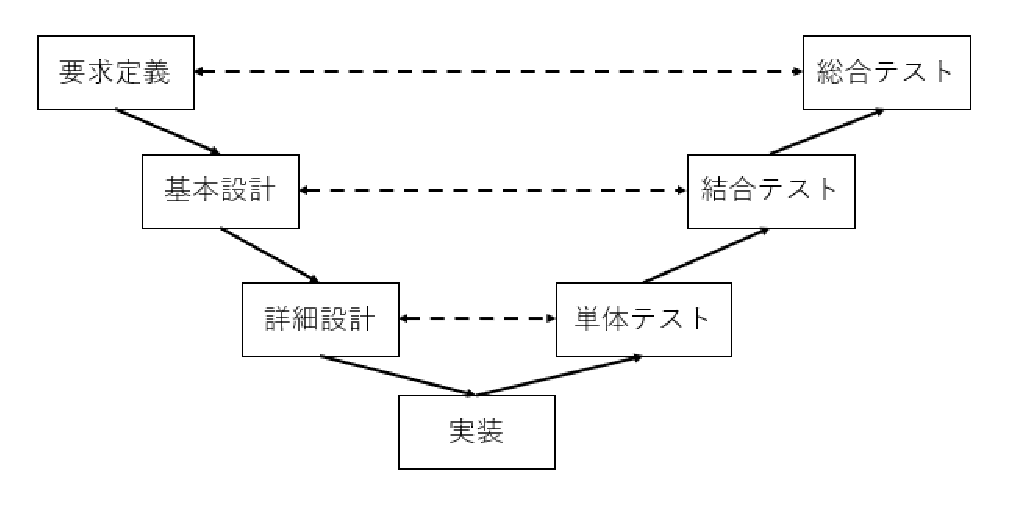
\includegraphics[height=60mm]{vmodel.eps}
	\caption{V字開発モデル}
        \label{fig:vmodel}
\end{center}
\end{figure}

%2章6節
\subsection{UML(Unified Modeling Language)}
UMLとは,オブジェクト指向分析,
設計においてシステムをモデル化する際の記法を規定した言語である.
UMLの用途は,プログラムを書く前に図で考えを整理すことや,
チーム開発において図でコミュニケーションをとること,
ユーザーや顧客と仕様を検討するなどの場合である\cite{uml}.

\subsection{ユースケース図}
ユースケース図とは,システムの仕様機能(ユースケース)と,外部環境(アクター)との関連を表す\cite{uml}.
一目でシステムの機能やシステム外部と内部の境界を理解することができるため,
ユーザーとクライアントとの意識統一を図ることが容易になる.
ユースケース図において,ユースケースはシステムの使用機能を楕円の中にユースケース名として記述する.
アクターは,機能を利用するユーザーや,システムが使用するハードウェア,外部システムを表現する.

\subsection{シーケンス図}
シーケンス図とは,オブジェクトの相互作用を表す相互作用図の一つで,
オブジェクト間のメッセージのやりとりを,時系列に沿って表現する\cite{uml}.

\subsection{クラス図}
クラス図とは,モデルの静的な構造を表し,システムの構造を表現できる\cite{uml}.
パッケージ単位の表現や,全体での表現,または,機能単位での表現など,様々な視点で作成することができる.


\chapter{SAS-L2認証方法}

本章では,SAS-L2での認証方法について説明する.
\section{SAS-L2(SimpleAnd Secure password authentication protocol,Light processing version, type 2)の概要}
SAS-L2とは,高知工科大学の清水明宏教授が提案した処理負荷が特に小さいワンタイムパスワード認証方式SAS-Lの一つである\cite{sas-l}.
表\ref{tb:sashikaku}から分かるように,従来のSASと比較し,特に被認証者側の処理負荷が小さい認証方式である.

\begin{table}[H]
\centering
\caption{SAS-2とSAS-L2の演算回数の比較}
\label{tb:sashikaku}
\begin{tabular}{|c|c|c|c|c|c|c|} \hline
 & \multicolumn{3}{c|}{ユーザー} & \multicolumn{3}{c|}{サーバー} \\
 \cline{2-7}
  & ハッシュ関数 & XOR & 加算 & ハッシュ関数 & XOR & 加算\\ \hline
  SAS-2 & 2 & 3 & 0 & 1 & 2 & 0\\ \hline
  SAS-L2 & 0 & 2 & 2 & 1 & 3 & 2\\ \hline
  \end{tabular}
  \end{table}

処理性能の低いIoT機器において,極めて小さい処理負荷で暗号鍵の配送が実現できる.
バーナム暗号などと組み合わせて暗号系を組むことで,処理能力の低いIoT機器へ暗号化通信機能を付加できる\cite{sas-l}.
SAS-L2は,認証者と被認証者にあらかじめ初回認証情報と初回秘匿情報の登録を行う初期登録処理と,
以降の認証処理から構成される.
認証者と被認証者は,以降でそれぞれサーバー,ユーザーと定義する.


\subsection{初期登録処理}
SAS-L2の初期登録処理のフローチャートを図\ref{fig:sas-l2_syoki}に示す.

\begin{figure}[H]
\begin{center}
	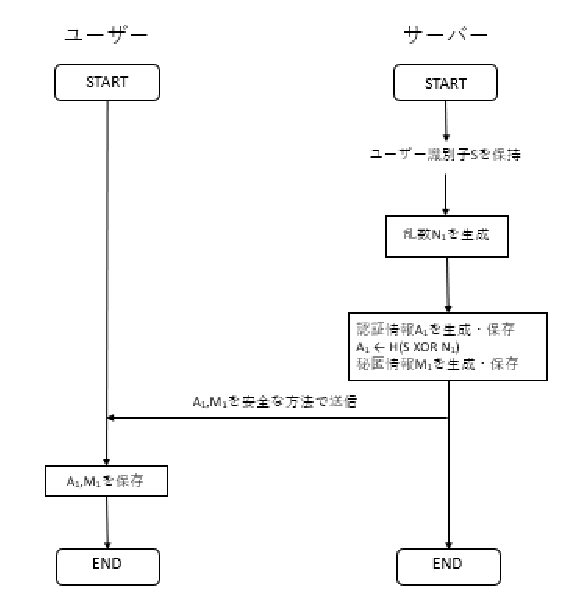
\includegraphics[height=100mm]{sas_l2_syoki.eps}
	\caption{初期登録処理の手順}
\label{fig:sas-l2_syoki}
\end{center}
\end{figure}

初期登録は,以下の手順に沿って処理が行われる.
\begin{enumerate}
	\item サーバーはユーザー識別子$S$を保持する.
	\item サーバーは初期認証用の乱数$N_1$を生成する.
	\item サーバーは,ユーザー識別子$S$と乱数$N_1$の排他的論理和にハッシュ関数を適用し,
	初期認証用の認証情報$A_1$を生成・保存する.
	\item サーバーは初期認証用の秘匿情報$M_1$を生成・保存する.
	\item サーバーは認証情報$A_1$と秘匿情報$M_1$を安全な方法でユーザーに送信する.
	\item ユーザーはサーバーから受信した認証情報$A_1$と秘匿情報$M_1$を保存する.
\end{enumerate}
初期登録の終了後,以降は認証処理が行われる.

\subsection {認証処理}
SAS-L2の$n$回認証時のフローチャートを図\ref{fig:sas-l2_ninsyo}に示す.
$N_n$,$A_n$,$M_n$はそれぞれ$n$回目認証用の乱数,認証情報,秘匿情報である.

\begin{figure}[H]
\begin{center}
	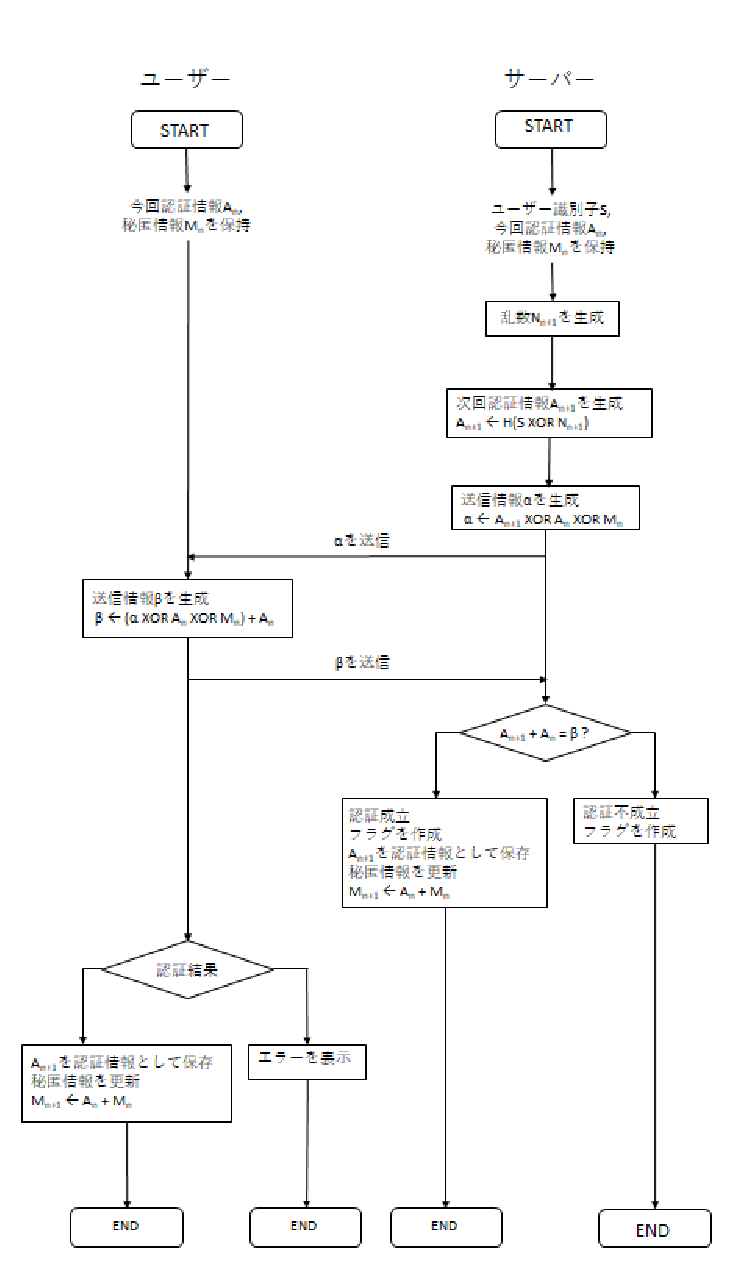
\includegraphics[height=200mm]{sas_l2.eps}
	\caption{認証手順}
\label{fig:sas-l2_ninsyo}
\end{center}
\end{figure}

認証は,以下の手順に沿って処理が行われる.
\begin{enumerate}
	\item サーバーはユーザー識別子$S$と認証情報$A_n$と秘匿情報$M_n$を保持している.
	ユーザーは認証情報$A_n$と秘匿情報$M_n$を保持している.
	\item サーバーは次回認証用の乱数$N_{n+1}$を生成する.
	\item サーバーは,ユーザー識別子$S$と乱数$N_{n+1}$の排他的論理和にハッシュ関数を適用し,
	次回認証用の認証情報$A_{n+1}$を生成する.
	\item サーバーは認証情報$A_{n+1}$,$A_n$と秘匿情報$M_n$の排他的論理和を演算し,$\alpha$を生成する.
	\item サーバーは$\alpha$をユーザーに送信する.
	\item ユーザーはサーバーから受信した$\alpha$と認証情報$A_n$,秘匿情報$M_n$の排他的論理和($\alpha \oplus A_n \oplus M_n(=A_{n+1})$)
	と認証情報$A_n$の算術加算により,$\beta$を生成する.
	\item ユーザーは$\beta$をサーバーに送信する.
	\item サーバーはユーザーから受信した認証情報$A_{n+1}$と保持していた$A_n$の加算を$\beta$と比較し,
	一致すれば認証成功し以下の処理が実行される.不一致ならば認証は不成立となり,
	以下の処理は実行されない.
	\item ユーザーは$\alpha$と認証情報$A_n$,秘匿情報$M_n$の排他的論理和を演算し次回認証用の認証情報$A_{n+1}$を生成し保存する.
	認証情報$A_n$と秘匿情報$M_n$の加算を行い,次回認証用の秘匿情報$M_{n+1}$を$M_n$の代わりに保存する.
\end{enumerate}
以上の処理で1回の認証が終了し,次回以降も認証を行う度に以上の処理を繰り返す.


\chapter{センシングデータ通信の暗号化}
%第3章:暗号化手法

本章では,SAS-L2に基づいたデータ通信の暗号化について説明する.
%3章1節
\section{SAS-L2に基づいたデータ通信の暗号化}
本研究では,SAS-L2ワンタイムパスワード認証方式に基づいたセンシングデータ通信の暗号化方法を提案し,
IoTシステムにおいてセンシングデータの暗号化通信を実現させる.
暗号化通信における送信側のセンシングデータの暗号化と
受信側のセンシングデータの復号化のアルゴリズムを説明する.

\subsection{送信側のセンシングデータ暗号化}
アルゴリズム1は,センシングデータを送信するエッジデバイス側の暗号化アルゴリズムである.
$n$回目とは,その時点までに行った提案手法による暗号化通信の回数とする.
以降,エッジデバイスはユーザーと定義する.

ユーザーは初めに,アルゴリズム1の処理1のようにセンシングデータ($SD$)と認証情報$A_{n+1}$,$A_n$の排他的論理和を演算し$\gamma$を生成する.
処理2では,$\gamma$をサーバーに送信する.
処理3では,$\alpha$をサーバーから受信する.
処理4では,$\alpha$と認証情報$A_{n+1}$と秘匿情報$M_{n+1}$の排他的論理和を演算し,$A_{n+2}$の復号化を行う.
処理5では,認証情報$A_{n+1}$と秘匿情報$M_{n+1}$の算術加算により,秘匿情報$M_{n+2}$を生成する.
処理6では,認証情報$A_n$,$A_{n+1}$と秘匿情報$M_{n+1}$を更新する.
処理1から処理6までを1回のエッジデバイス側でのデータ暗号化とし,10回の繰り返しを終えたら,処理7で認証情報$A_n \leftarrow A_{n+1}$,秘匿情報$M_n \leftarrow M_{n+1}$として保存する.
\begin{algorithm}[H]
\caption{$n$回目のエッジデバイス側でのデータ暗号化}
\begin{algorithmic}[1]
\renewcommand{\algorithmicrequire}{\textbf{Input:}}
\renewcommand{\algorithmicensure}{\textbf{Output:}}
\REQUIRE $\alpha$,$SD$,$n$回目認証情報$A_n$,$n+1$回目認証情報$A_{n+1}$,$n+1$回目秘匿情報$M_{n+1}$
\ENSURE $\gamma$
\STATE $\gamma \leftarrow SD \oplus A_{n+1} \oplus A_n$
\STATE $\gamma$をサーバーに送信
\STATE $\alpha$をサーバーから受信
\STATE $A_{n+2} \leftarrow \alpha \oplus A_{n+1} \oplus M_{n+1}$
\STATE $M_{n+2} \leftarrow A_{n+1} + M_{n+1}$
\STATE 認証情報$A_n$,$A_{n+1}$と秘匿情報$M_{n+1}$を更新.
\\ $A_n \leftarrow A_{n+1}$
\\ $A_{n+1} \leftarrow A_{n+2}$
\\ $M_{n+1} \leftarrow M_{n+2}$
\STATE 処理1から6まで10回繰り返した後,認証情報$A_n \leftarrow A_{n+1}$,秘匿情報$M_n \leftarrow M_{n+1}$として保存.
\end{algorithmic} 
\end{algorithm}


\subsection{受信側のセンシングデータの復号化}

アルゴリズム2は,センシングデータを受信するサーバー側の復号のアルゴリズムである.
$n$回目とは,その時点までに行った提案手法による暗号化通信の回数とする.
以降,エッジデバイスはユーザーと定義する.


サーバーは初めに,アルゴリズム2の処理1のように送信者であるユーザーから,センシングデータ($SD$)を暗号化した$\gamma$を受信する.
処理2では,$\gamma$と認証情報$A_{n+1}$,$A_n$の排他的論理和を演算し,$SD$を復号化する.
処理3では,乱数$N_{n+2}$を生成し,
処理4で乱数$N_{n+2}$とユーザー識別子$S$の排他的論理和にハッシュ関数を適用することで,次回認証情報$A_{n+2}$を生成する.
処理5では,認証情報$A_{n+2}$,$A_{n+1}$と秘匿情報$M_{n+1}$の排他的論理和を演算し,$\alpha$を生成する.
処理6では,$\alpha$をユーザーに送信する.
処理7では,認証情報$A_{n+1}$と秘匿情報$M_{n+1}$の算術加算により,秘匿情報$M_{n+2}$を生成する.
処理8では,認証情報$A_n$,$A_{n+1}$と秘匿情報$M_{n+1}$を更新する.
処理1から処理8までを1回のサーバーの暗号化データの復号とし,10回の繰り返しを終えたら,処理9で認証情報$A_n \leftarrow A_{n+1}$,秘匿情報$M_n \leftarrow M_{n+1}$として保存する.
\begin{algorithm}[H]
\caption{n回目のサーバーの暗号化データの復号}
\begin{algorithmic}[1]
\renewcommand{\algorithmicrequire}{\textbf{Input:}}
\renewcommand{\algorithmicensure}{\textbf{Output:}}
\REQUIRE $\gamma$,ユーザー識別子$S$,$n$回目認証情報$A_n$,$n+1$認証情報$A_{n+1}$,$n+1$秘匿情報$M_{n+1}$
\ENSURE $\alpha$,$SD$
\STATE $\gamma$をユーザーから受信
\STATE $SD \leftarrow \gamma \oplus A_{n+1} \oplus A_n$
\STATE 乱数$N_{n+2}$を生成
\STATE $A_{n+2} \leftarrow H(S \oplus N_{n+2})$
\STATE $\alpha \leftarrow A_{n+2} \oplus A_{n+1} \oplus M_{n+1}$
\STATE $\alpha$をユーザーに送信
\STATE $M_{n+2} \leftarrow A_{n+1} + M_{n+1}$
\STATE 認証情報$A_n$,$A_{n+1}$と秘匿情報$M_{n+1}$を更新.
\\ $A_n \leftarrow A_{n+1}$
\\ $A_{n+1} \leftarrow A_{n+2}$
\\ $M_{n+1} \leftarrow M_{n+2}$
\STATE 処理1から8まで10回繰り返した後,認証情報$A_n \leftarrow A_{n+1}$,秘匿情報$M_n \leftarrow M_{n+1}$として保存.
\end{algorithmic} 
\end{algorithm}


\subsection{提案手法の利点}
 第2章で述べたように,従来暗号方式としてバーナム暗号がある.
 バーナム暗号では,鍵は一度しか使用することができず,暗号化を行う度に鍵を共有する必要があり,
 鍵を共有する毎に鍵が直接ネットワークに流れるという欠点がある.
 これに対して,提案手法のSAS-L2に基いたデータ通信の暗号化方法では,鍵を共有する際に,鍵が直接ネットワークに流れないという利点がある.
 例えば,1回目の暗号化通信では,鍵として認証情報$A_2$と認証情報$A_1$が必要となる.
 認証情報$A_1$は,IoTエッジデバイスに初期認証情報として秘匿情報$M_1$と共に書き込まれているとすれば,
 認証者が被認証者に認証情報を送信する必要がなくなる.
 認証情報$A_2$は,認証者が被認証者に送信することで共有するが,
 認証情報$A_1$と秘匿情報$M_1$を持っていなければ認証情報$A_2$を復号することができない.
 このように,提案手法では鍵と認証情報と秘匿情報の排他的論理和を演算して送信することから,鍵がそのままネットワークに流れることなく鍵を配送できる.


また,第2章で述べた従来の暗号化方式であるAESは,暗号化したいデータを,ブロックに分け,ブロック毎に4種類の変換を複数回繰り返すことで暗号化が行われる.このように,AESなどの従来の暗号化方式は暗号化での処理負荷が大きい.これに対して,提案手法では暗号化を行いたいデータと認証情報$A_n$と$A_{n+1}$との排他的論理和を演算し,第3章で説明したSAS-L2の認証アルゴリズムと同様に鍵を更新することで暗号化通信ができる.このように,従来の暗号化方式と比較して提案手法は処理負荷が小さく,処理性能の低いIoTセンシングデバイスへの実装が実現できる.


\chapter{SAS-L2を用いたセキュアな組込みシステムの開発}
%第4章:システム仕様

本章では,SAS-L2を用いたセキュアな組込みシステムについての仕様を述べる.

\section{SAS-L2を用いたセキュアな組込みシステムの概要}
はじめに,SAS-L2を利用したセキュアな組込みシステムの概要図を図\ref{fig:gaiyo}示す.

\begin{figure}[H]
\begin{center}
	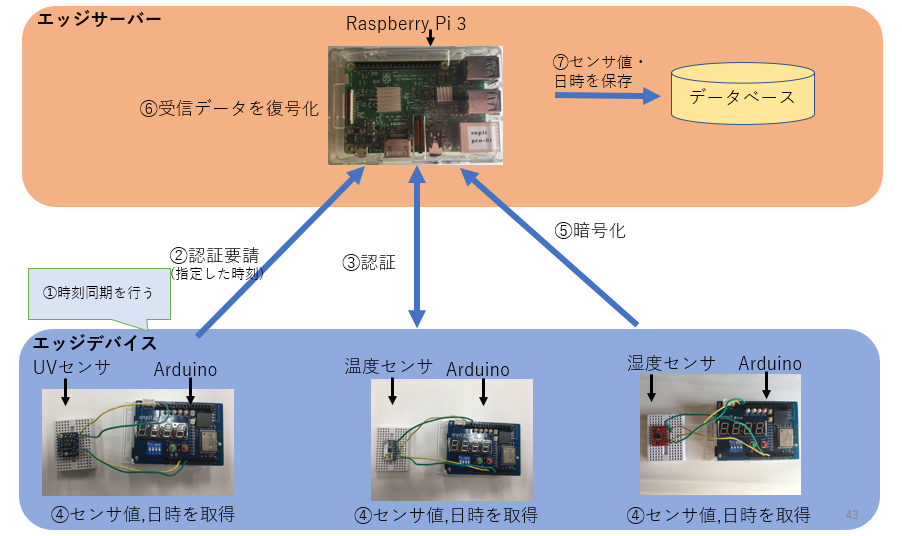
\includegraphics[height=80mm]{gaiyo.png}
	\caption{SAS-L2を利用したセキュアな組込みシステムの概要図}
\label{fig:gaiyo}
\end{center}
\end{figure}

Raspberry Piをエッジサーバーとし,3台のArduinoをエッジデバイスとして利用する.
図\ref{fig:gaiyo}のように,エッジデバイスにはそれぞれ,UVセンサ,温度センサ,湿度センサを接続している.
データベースには,エッジデバイスから収集したデータを保存する.
以降,エッジサーバーをサーバー,エッジデバイスをユーザーと定義する.
図\ref{fig:gaiyo}に沿って,SAS-L2を利用したセキュアな組込みシステムの時刻同期,センシングデータ取得,認証,および暗号化通信の処理の流れを説明する.

\begin{enumerate}
	\item ユーザーを起動し,時刻同期を行う.
	\item ユーザーはサーバーに対して,指定した時刻に認証要請を行う.
	\item サーバーは認証要請を受信し,認証要請を送信したユーザーとのSAS-L2認証を行う.
	\item ユーザーは認証完了後,接続されたセンサからセンシングデータ(センサ値)と,
    センシングデータを取得した日時を取得する.
	\item ユーザーは処理4で取得したデータを暗号化しサーバーへ送信する.
	\item サーバーはユーザーから受信したデータを復号し,センシングデータと日時を取得する.
    \item サーバーは取得した,センシングデータと日時をデータベースに保存する.
    \item 処理4から処理7を10回繰り返す.
    \item 処理2から処理8を繰り返す.
\end{enumerate} 

以上のように,指定した時刻になると認証1回,暗号化通信10回を行うシステムとなる.

\section{要件定義}
SAS-L2を利用したセキュアな組込みシステムの要件定義を述べる.
要件定義には,機能要件と非機能要件がある.
機能要件は,システムで実現すべき機能であり,クライアントから求められる機能のことである.
非機能要件は,機能要件以外の要件であり,主に性能やセキュリティ,環境,制約を指す.
\subsubsection{機能要件}
\begin{enumerate}
	\item 指定した時刻にユーザ―からサーバーにコネクションして認証要請を送信する.
	\item サーバーとユーザー間でSAS-L2による認証を行う.
    \item 認証が成功した場合,サーバーとユーザー間でSAS-L2に基づいた暗号化通信を行う.
    \item 認証が失敗した場合,コネクションを切断してシステム概要で述べた処理1からやり直す.
	\item サーバーは受信データを復号してセンシングデータと日時をデータベースへ保存する.
    \item 暗号化通信終了後,サーバーはコネクションを切断し,ユーザーからの認証要請待ち状態となる.
\end{enumerate} 

\subsubsection{非機能要件}
\begin{enumerate}
    \item 複数のユーザーは同時刻に認証要請を送信するので,一台の認証が終了するまで,その他のユーザーは待機状態になる.
    \item サーバーは認証結果をユーザーに送信する.
    \item サーバーとユーザーは認証結果を表示する.
    \item ユーザーは,シリアルモニタに取得したセンシングデータとセンシングデータの取得日時を表示する.
    \item ユーザーは起動後,1度時刻同期を行う.
    \item サーバーは暗号化通信の際,5秒以上データを受信できなければ,コネクションを切断し,認証要請受信の待機状態となる.
	\item 指定した時刻毎に3つのユーザーとの通信を10秒以内に終わらせる.
    \item サーバーはセンシングデータと取得日時を保存する際に,ユーザーごとのテーブルに分けて保存する.
    \item 1度の認証につき,10回の暗号化通信を行う.
	\item ユーザーで,何らかのエラーが発生した場合,赤LEDを点滅させる.
\end{enumerate} 


\chapter{SAS-L2を用いたセキュアな組込みシステムの設計}
%システム設計

本章では,SAS-L2を利用したセキュアな組込みシステムについての設計を述べる.
システム開発にあたり,基本設計の作成と役割分担,スケジュールの決定,詳細設計とテスト項目を作成した.
基本設計と詳細設計はUMLを用いて行った.

\section{基本設計}
基本設計では,ユースケース図とクラス図とシーケンス図を作成した.
\begin{figure}[H]
\begin{center}
	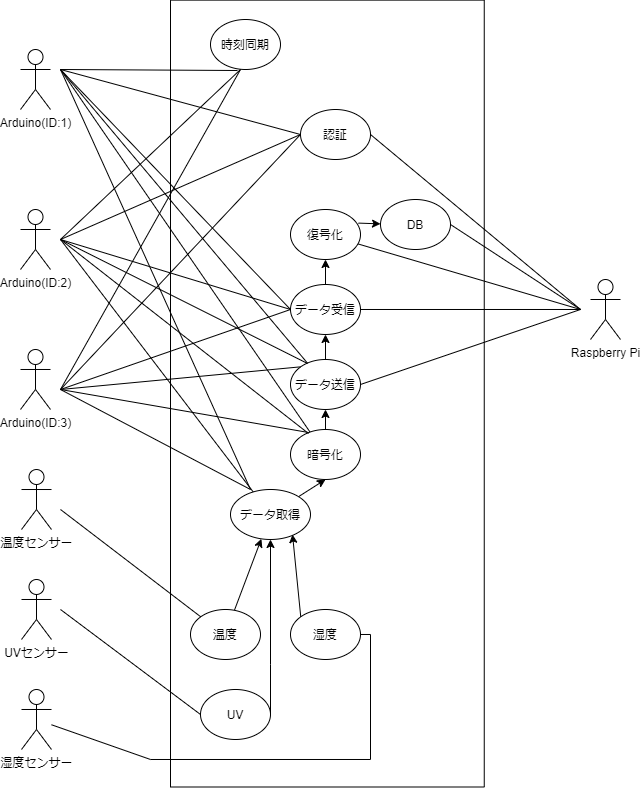
\includegraphics[width=10cm]{usecase.png}
	\caption{ユースケース図}
	\label{fig:kihon_usecase}
\end{center}
\end{figure}

図\ref{fig:kihon_usecase}のユースケース図では,システム内の基本機能を視覚的に図示している.
ユースケース図の作成により,システムの機能の洗い出しや役割分担を決定した.

\begin{figure}[H]
\begin{center}
	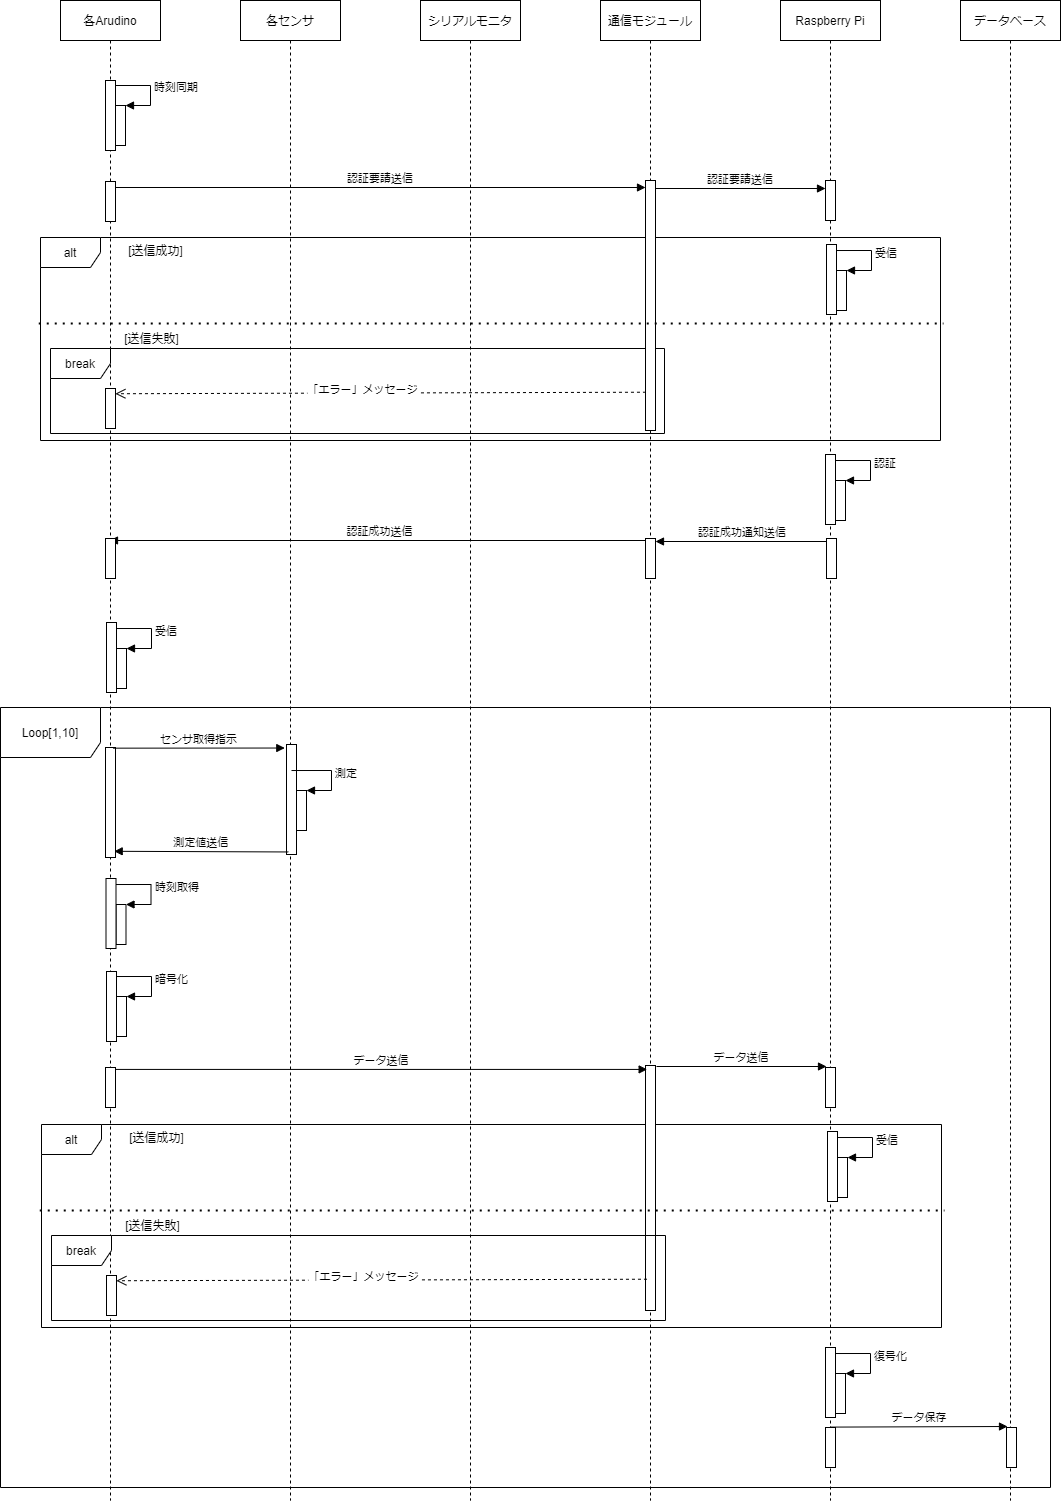
\includegraphics[height=200mm]{kihon_sequence.png}
	\caption{シーケンス図}
	\label{fig:kihon_sequence}
\end{center}
\end{figure}
図\ref{fig:kihon_sequence}のシーケンス図では,クラス間で行われる処理を時系列で表している.
初めに,Arduinoが時刻同期を行う.
次に,Arduinoから通信モジュールを経由してRaspbery Piへ認証要請を行う.
Arduinoが送信成功すればRaspbery Piは認証要請を受信し,送信失敗した場合は
通信モジュールからエラーメッセージが送信され,処理が中断される.
その後,Raspbery Piにより認証を行い,認証成功通知をArduinoへ送信する.
認証処理終了後,Arduinoは接続されているセンサからセンシングデータと,
センシングデータを取得した日時を取得し,暗号化を行う.
Arduinoは暗号化したデータをRaspbery Piへ送信し,
送信成功すればRaspbery Piはデータを受信し,送信失敗した場合は
通信モジュールからエラーメッセージが送信され,処理が中断される.
最後にRaspbery Piが受信したデータを復号し,得られたセンシングデータと
センシングデータの取得日時をデータベースへ保存する.
図\ref{fig:kihon_sequence}に示されているLoop[]はループと言い,[]内で示された範囲での繰り返し処理が行われる.
ここではLoop[1,10]であることから,10回の繰り返し処理が行われる.

\begin{figure}[H]
\begin{center}
	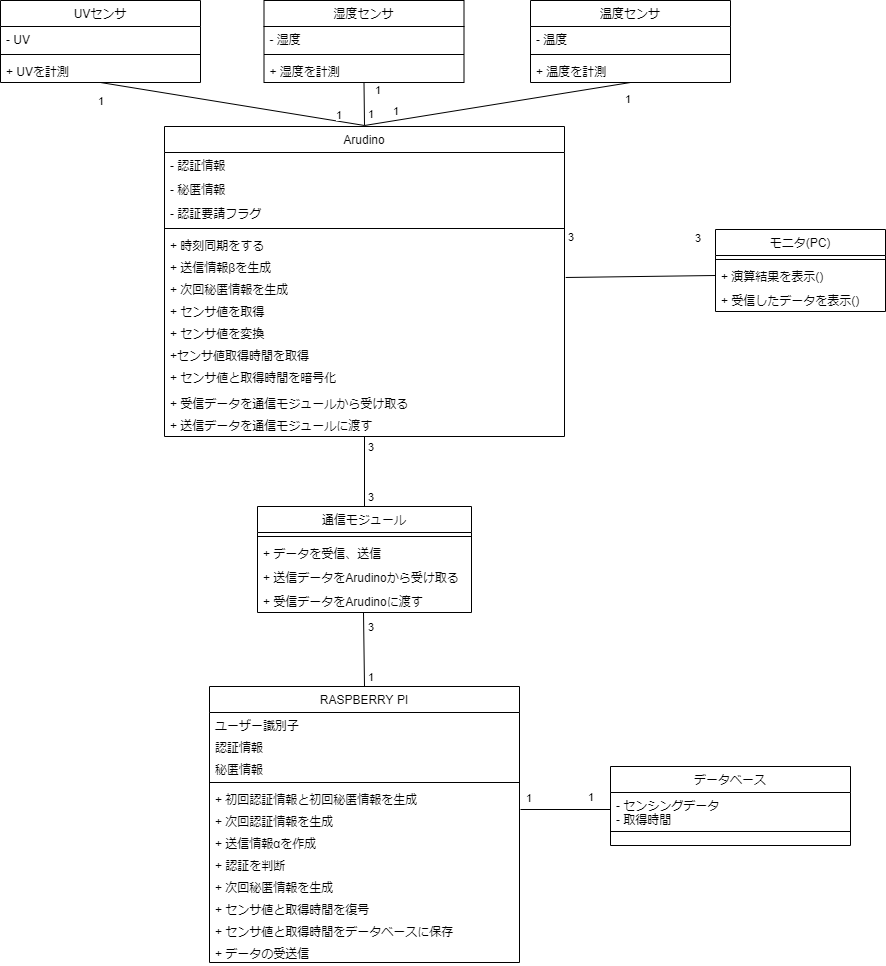
\includegraphics[height=140mm]{kihon_class.png}
	\caption{クラス図}
	\label{fig:kihon_class}
\end{center}
\end{figure}
図\ref{fig:kihon_class}のクラス図では,システムの静的な構造と関係性を視覚的に表している.
温度センサ,湿度センサ,UVセンサ,Arduino,モニタ,通信モジュール,Raspbery Pi,データベースをクラスとしている.
関連のあるクラス間での多重度も示している.

\section{役割分担}
図\ref{fig:kihon_usecase}のユースケース図から,役割分担を行った.
Arduinoの時刻同期とセンサからのセンシングデータ取得,データを暗号化しRaspbery Piへ送信する機能を浅野が担当した.
Raspbery PiのArduinoからのデータ受信とデータの復号化,データベースへの保存を内山田が担当した.
認証については,被認証側を浅野,認証側を内山田が担当した.

\section{スケジュール}
スケジュール管理は,ガントチャートで行った.
図\ref{fig:ganto}のようにガントチャートをEXCELで作成し,チーム内で共有しながら進捗を管理した.

\begin{figure}[H]
\begin{center}
	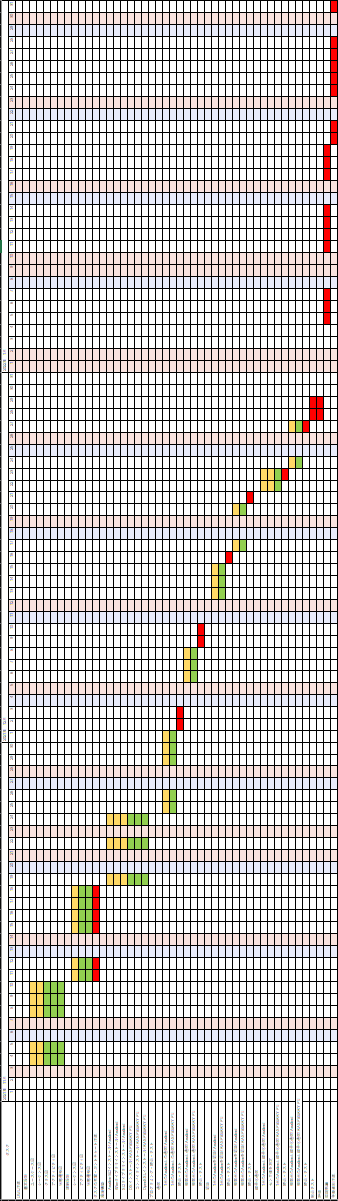
\includegraphics[height=220mm]{ganto.png}
	\caption{ガントチャート}
	\label{fig:ganto}
\end{center}
\end{figure}



\section{詳細設計}
担当する機能についての詳細設計をUMLを用いて行い,時間同期,認証における被認証者の処理,センシングデータの取得,暗号化通信についてのシーケンス図を作成した.
また,暗号化通信における通信フォーマットの定義も行った.

\begin{figure}[H]
\begin{center}
	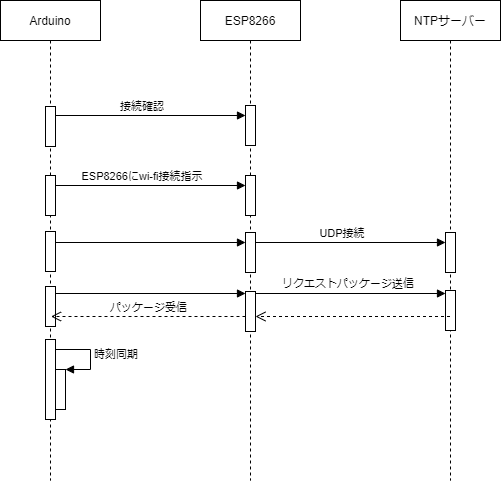
\includegraphics[height=80mm]{time_sequence.png}
	\caption{時間同期におけるシーケンス図}
	\label{fig:time_sequence}
\end{center}
\end{figure}
図\ref{fig:time_sequence}のシーケンス図では,Arduinoにおける時刻同期に関するクラス間で行われる処理を時系列で表している.
初めに,Arduinoが通信モジュールであるESP8266との接続を行う.
次に,Arduinoは通信モジュールを介してWi-Fiとの接続を行う.
日時を取得するために,ArduinoからNTPサーバーにUDP接続し,リクエストパッケージを送信する.
そして,NTPサーバーから受信したパッケージより,日時を取得して時刻同期を行う.
時刻同期の完了後,SAS-L2による認証・暗号化通信が行われる.

\begin{figure}[H]
\begin{center}
	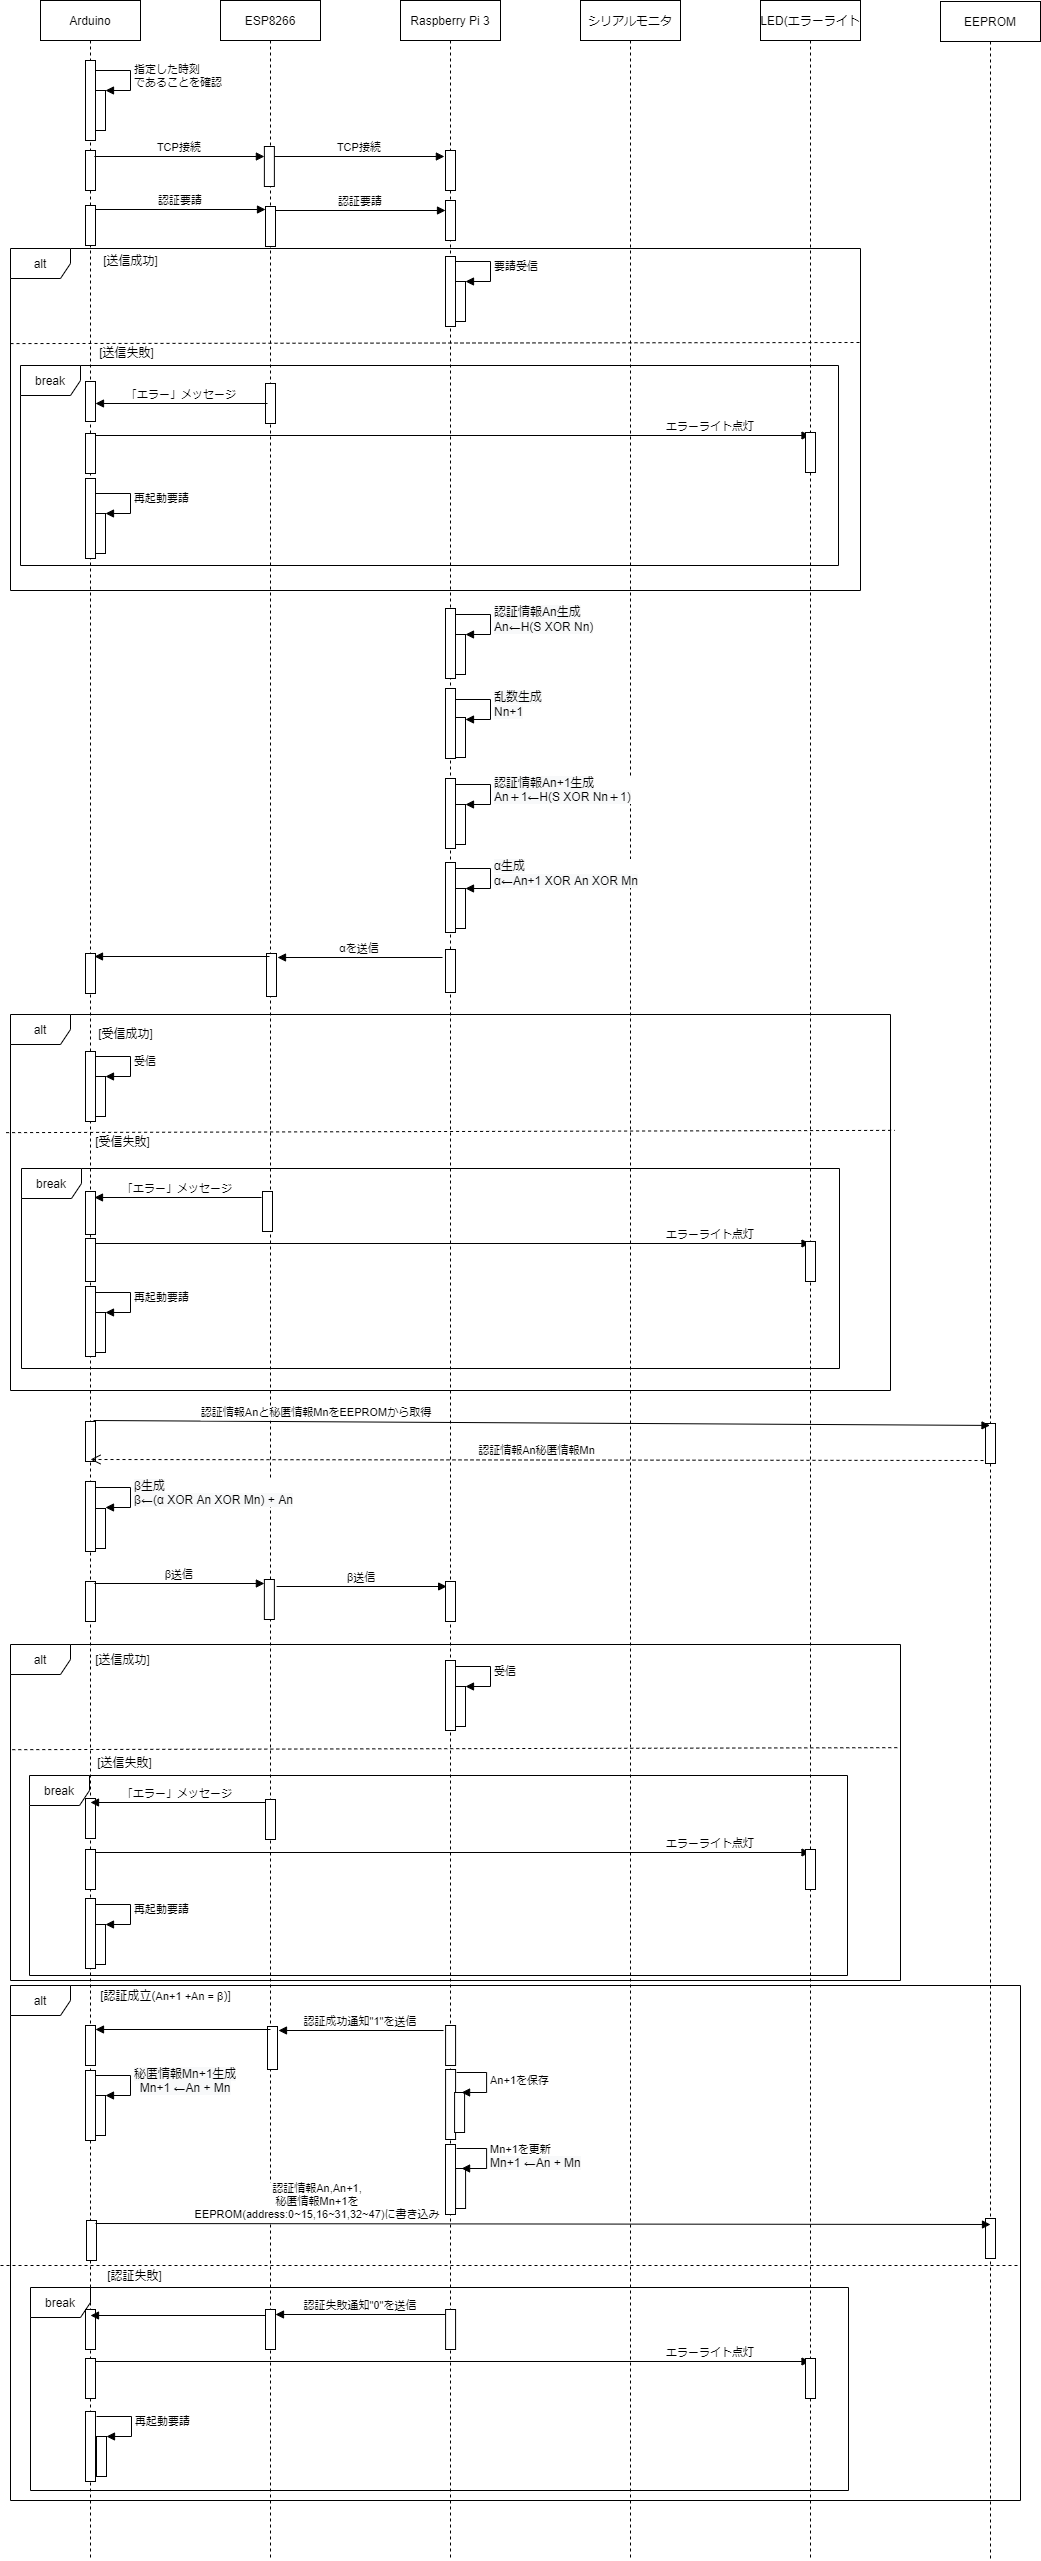
\includegraphics[height=220mm]{ninsyo_sequence.png}
	\caption{認証におけるシーケンス図}
	\label{fig:ninsyo_sequence}
\end{center}
\end{figure}

図\ref{fig:ninsyo_sequence}のシーケンス図では,Arduinoにおける認証に関するクラス間で行われる処理を時系列で表している.
初めに,Arduinoが指定した時刻になると,Raspberry Piに対してTCP接続を行い,認証要請を送信する.
認証要請が送信成功すれば以降の処理に進み,
送信失敗であれば通信モジュールであるESP8266からエラーメッセージがArduinoに対して送信され,
Arduinoの赤LEDが点滅し,利用者に対して再起動するように求める.
次に,Raspberry Piから$\alpha$を受信する.この時,受信が失敗すれば,
Arduinoの赤LEDが点滅し,利用者に対して再起動するように求める.
そして,ArduinoのEEPROMに書き込まれている認証情報と秘匿情報を読み出して,
$\beta$を生成し,Raspberry Piへ送信する.この時,送信が失敗すれば,
Arduinoの赤LEDが点滅し,利用者に対して再起動するように求める.
次に,認証結果をRaspberry Piから受信する.
認証成功なら"1"を受信して秘匿情報を生成し,更新した認証情報と秘匿情報をEEPROMに書き込む.
認証失敗なら"0"を受信して,Arduinoの赤LEDが点滅し,利用者に対して再起動するように求める.

\begin{figure}[H]
\begin{center}
	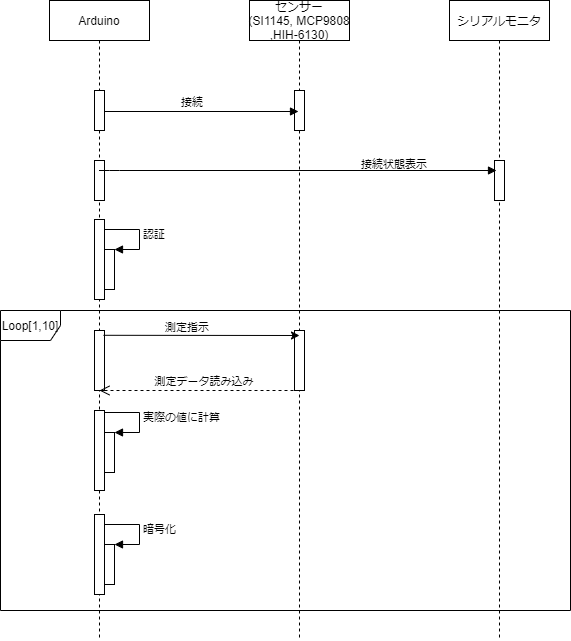
\includegraphics[height=100mm]{sensor_sequence.png}
	\caption{センシングデータ取得におけるシーケンス図}
	\label{fig:sensor_sequence}
\end{center}
\end{figure}

図\ref{fig:sensor_sequence}のシーケンス図では,
Arduinoにおけるセンシングデータ取得に関するクラス間で行われる処理を時系列で表している.
初めに,Arduinoは接続されているセンサと接続を行い,
確認のためにシリアルモニタへセンサとの接続状態を表示する.
次に,認証完了後,Arduinoはセンサへ測定指示を出して測定値を取得する.
取得した測定値を実際の値へと変換するために計算を行う.
計算後の値をセンシングデータとし,そのセンシングデータを利用して暗号化通信を行う.
図\ref{fig:sensor_sequence}に書かれているLoop[1,10]の部分では,10回の繰り返し処理が行われる.

\begin{figure}[H]
\begin{center}
	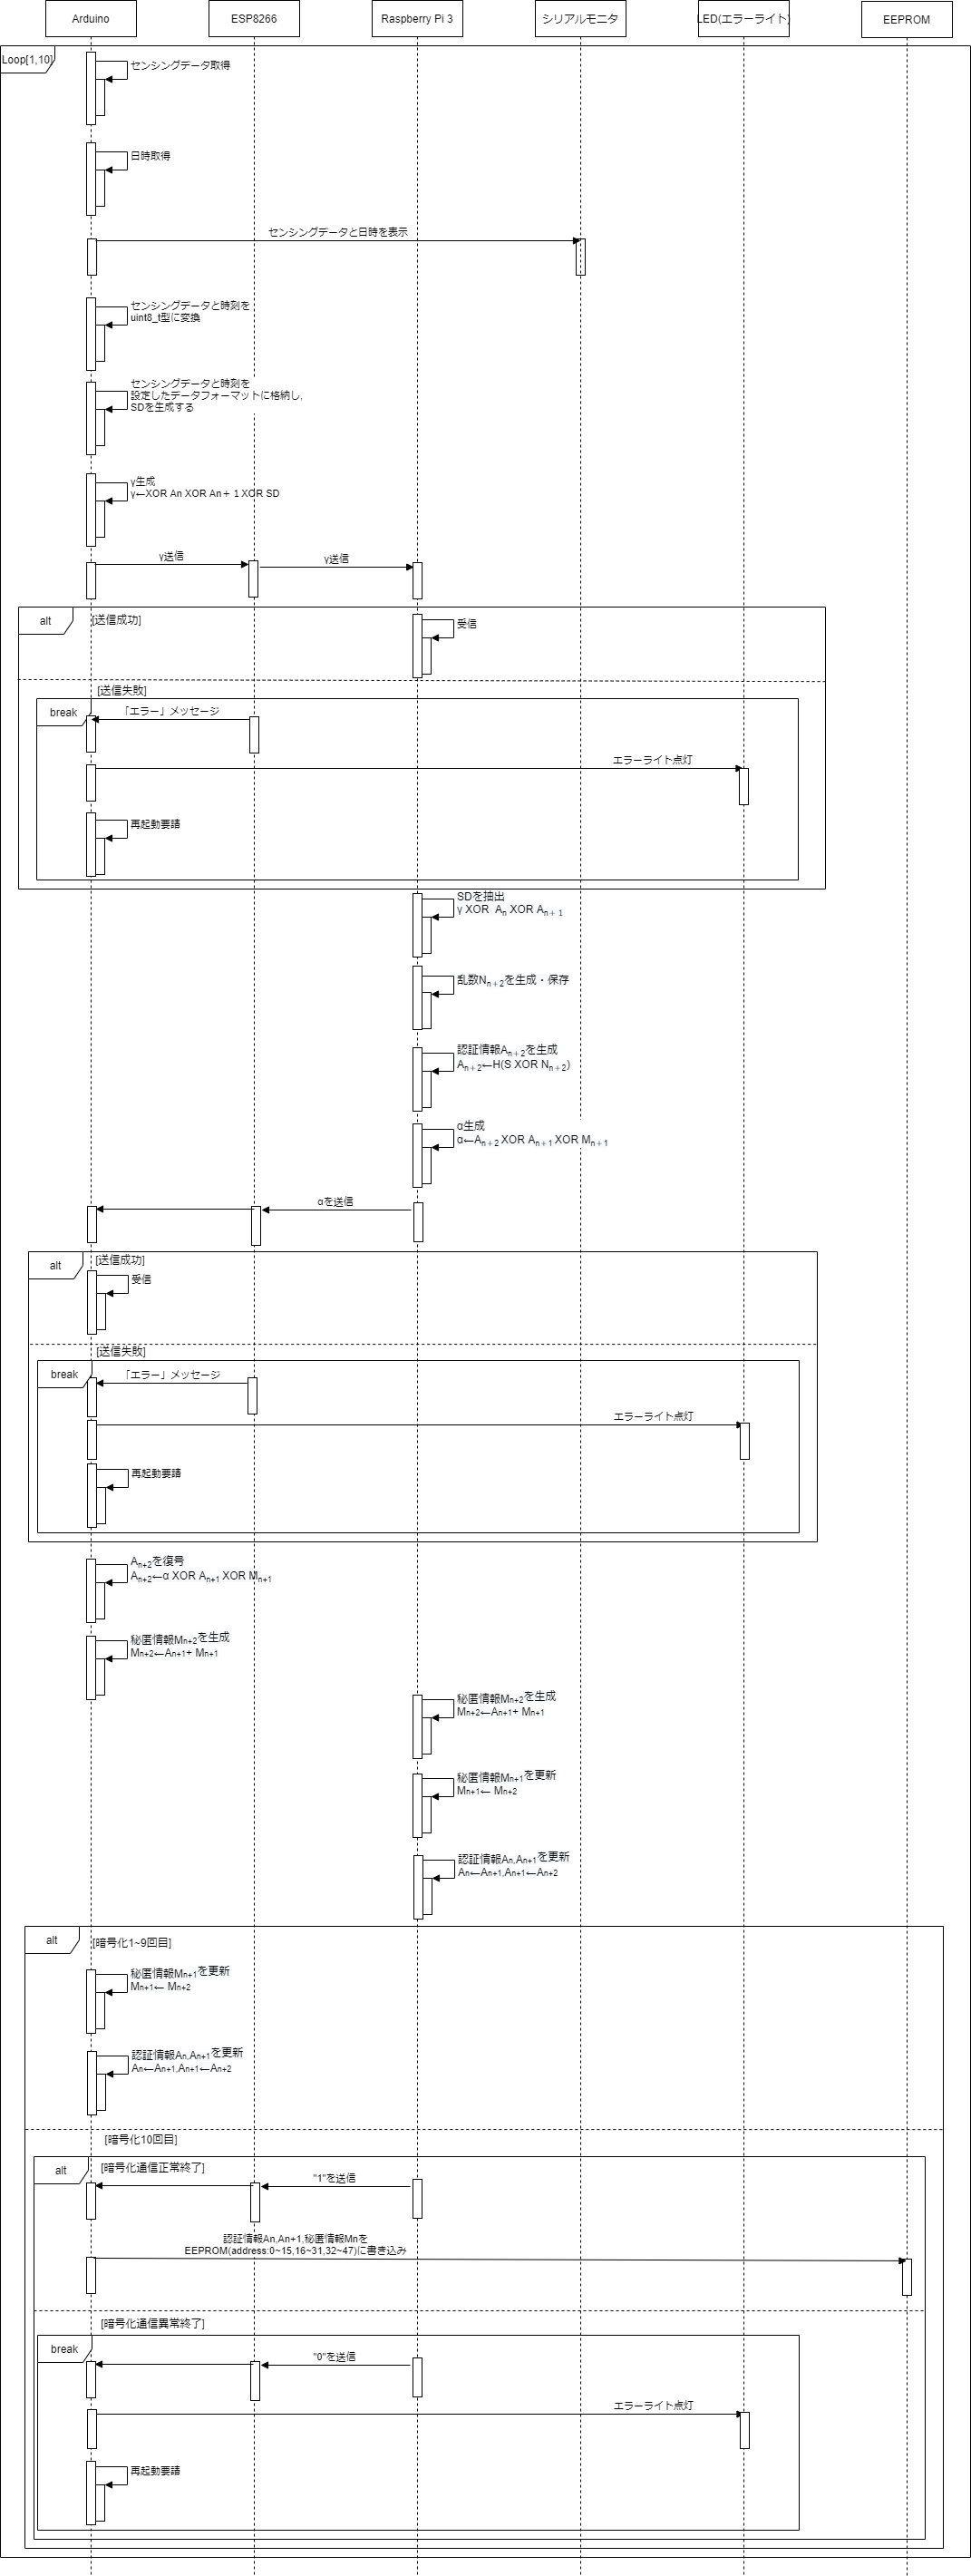
\includegraphics[height=200mm]{ango_sequence.png}
	\caption{暗号化通信におけるシーケンス図}
	\label{fig:ango_sequence}
\end{center}
\end{figure}

図\ref{fig:ango_sequence}のシーケンス図では,
Arduinoにおける暗号化通信に関するクラス間で行われる処理を時系列で表している.
初めに,Arduinoはセンシングデータとセンシングデータを取得した日時を取得する.
そして,取得したセンシングデータと日時をシリアルモニタに表示する.
次に,取得したセンシングデータと日時をunsigned char型へ変換して,データフォーマットに格納し$SD$を生成する.
そして,生成した$SD$を利用して$\gamma$を生成し,Raspberry Piへ送信する.この時,送信が失敗すれば,
Arduinoの赤LEDが点滅し,利用者に対して再起動するように求める.
次に,Raspberry Piから$\alpha$を受信する.この時,受信が失敗すれば,
Arduinoの赤LEDが点滅し,利用者に対して再起動するように求める.
受信した$\alpha$から次回認証情報を復号し,その後,次回秘匿情報を生成する.
最後に,認証情報と秘匿情報の更新を行う.
暗号化通信が1から9回目の場合は,認証情報と秘匿情報を格納している配列を更新する.
暗号化通信が10回目の場合,正常に暗号化通信が終了した時はRaspberry Piから"1"を受信し,
更新した認証情報と秘匿情報をEEPROMに書き込む.
暗号化通信が正常に終了しなかった時は,Raspberry Piから"0"を受信して,
Arduinoの赤LEDが点滅し,利用者に対して再起動するように求める.

%%\begin{figure}[h]
%%\begin{center}
%%	\includegraphics[height=40mm]{syosai_class.eps}
%%	\caption{クラス図}
%%\end{center}
%%\end{figure}

\subsection{データフォーマット}
暗号化通信の際に,$\gamma \leftarrow SD \oplus  A_{n+1} \oplus A_n$の演算によって$\gamma$を生成する.
$\gamma$の生成には$SD$が必要となり,この$SD$にはセンシングデータとセンシングデータを取得した日時が格納されている.
ArduinoとRaspberry Pi間では,基本的にunsigned char型の128bit配列でデータの送受信が行われるため,
センシングデータと日時をunsigned char型の16byte(128bit)配列$SD$に格納するためにデータフォーマットを作成した.作成したデータフォーマットを図\ref{fig:format}に示す.
まず,センシングデータはfloat型で取得される.float型は32bitであることから,センシングデータのビット列は配列$SD$[0]から$SD$[3]に格納する.
次に,日時の内容は年,月,日,時,分,秒である.年はint型の16bitで取得され,月,日,時,分,秒はそれぞれint型の8bitで取得される.
このことから,年のビット列は配列$SD$[4]から$SD$[5]に格納し,月のビット列は配列$SD$[6],日のビット列は配列$SD$[7],
時のビット列は配列$SD$[8],分のビット列は配列$SD$[9],秒のビット列は配列$SD$[10]に格納される.
残りの配列$SD$[11]から$SD$[15]には乱数を設定し格納する.

\begin{figure}[H]
\begin{center}
	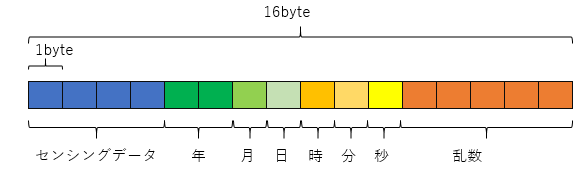
\includegraphics[height=30mm]{format.png}
	\caption{センシングデータと取得日時を格納する際のデータフォーマット}
	\label{fig:format}
\end{center}
\end{figure}

\section{テスト項目の作成}
本節では,本研究で作成した単体テスト項目と結合テスト項目,総合テスト項目について説明する.
\subsection{単体テスト項目}
単体テストではV字開発モデルに従って,詳細設計を参考し表\ref{tab:tantai_komoku}のテスト項目を作成した.
\begin{table}[H]
\centering
\caption{単体テスト項目}
\label{tab:tantai_komoku}
\scalebox{0.8}{
\begin{tabular}{|c|l|} \hline
 機能枠&確認内容\\ \hline\hline
 \multirow{2}{*}{通信モジュールとの接続} & 
  \shortstack[l]{
   ArduinoとESP8266を接続した時,ESP8266との接続が\\
   確認できたら,シリアルモニタに"ESP8266 OK"と表示\\
   される.}\\ \cline{2-2}
 & \shortstack[l]{
   ArduinoとESP8266を接続しなければ,ESP8266との\\
   接続が確認できず,赤LEDが点滅する.}\\ \hline
 Wi-Fi接続 &
   \shortstack[l]{
   Wi-Fiとの接続ができれば,シリアルモニタに"connect\\
   success"と 表示される.}\\ \hline
 UDP接続 &
   \shortstack[l]{
   IPアドレス"ntp.nict.jp",ポート番号"123"へUDP接続が\\
   成功すれば,時刻同期処理が開始される.}\\ \hline
 TCP接続 &
   \shortstack[l]{
   IPアドレス"192.168.2.110"、ポート番号"49152"へTCP\\
   接続が成功すれば, シリアルモニタに"create tcp ok"\\
   と表示される.}\\ \hline 
 \multirow{3}{*}{センサ} &
   Arduinoとセンサが接続している.\\ \cline{2-2}
 & \shortstack[l]{
   Arduinoとセンサが接続されていなければ赤LEDが点滅\\
   する.}\\ \cline{2-2}
 & センシングデータを取得する.\\ \hline
 時刻取得 &
   \shortstack[l]{
   センシングデータを取得した時点の年,月,日,時,分,秒\\
   を取得する.}\\ \hline
 \multirow{2}{*}{認証の際の$\beta$の演算} &
   \shortstack[l]{
   $\alpha \oplus A_n \oplus M_n$の演算結果が正しい.演算結果は128bit\\
   である.}\\ \cline{2-2}
 & \shortstack[l]{
   $\beta \leftarrow (\alpha \oplus A_n \oplus M_n )+A_n$の演算結果が正しい.\\
   演算結果は128bitである.}\\ \hline
 \shortstack[l]{ 
 認証の際の\\
 次回秘匿情報\\
 の計算} &
   \shortstack[l]{
   $M_{n+1} \leftarrow A_n + M_n$の演算が正しい.\\
   演算結果は128bitである.} \\ \hline
 \shortstack[l]{
 認証成功時の\\
 認証情報$A_n$,$A_{n+1}$,\\
 秘匿情報$M_n$の更新}
 & \shortstack[l]{
   n回目認証成功時の$A_n$,$A_{n+1}$,$M_{n+1}$をEEPROMのアドレス\\
   0-15,16-31,32-47にそれぞれ書き込む.}\\ \hline
 $SD$の生成 &
   \shortstack[l]{
   float型(32bit)センサ値と,int型(16bit)の年,int$8_t$型(8bit)\\
   の月,日,時,分,秒をunsigned char型の128bit配列に格納\\
   される.}\\ \hline
\shortstack[l]{
 暗号化通信の際の\\
$\gamma$の演算}&
   \shortstack[l]{
   $\gamma \leftarrow SD \oplus A_{n+1} \oplus A_n$ の演算結果が正しい.\\
   演算結果は128bitである.}\\ \hline
 \shortstack[l]{
 暗号化通信の際の\\
 認証情報$A_{n+2}$の演算} &
   \shortstack[l]{  
   $A_{n+2} \leftarrow \alpha \oplus A_{n+1} \oplus M_{n+1}$の演算結果が正しい.\\
   演算結果は128bitである.}\\ \hline
 \shortstack[l]{ 
 暗号化通信の際の\\
 次回秘匿情報の計算} &
   \shortstack[l]{
   $M_{n+2} \leftarrow A_{n+1} + M_{n+1}$の演算が正しい.演算結果は128bit\\
   である.}\\ \hline
 \shortstack[l]{ 
 暗号化通信の際の\\
 認証情報,\\
 秘匿情報の更新} &
   \shortstack[l]{   
   10回目暗号化終了時の$A_n$,$A_{n+1}$,$M_{n+1}$をEEPROMの\\
   アドレス0-15,16-31,32-47それぞれ書き込む.}\\ \hline
\end{tabular}
}
\end{table}

\subsection{結合テスト項目}
結合テストではV字開発モデルに従って,基本設計を参考し表\ref{tab:ketugo_komoku}のテスト項目を作成した.
Arduinoはユーザー,Raspberry Piはサーバーと定義する.


\begin{table}[H]
\centering
\caption{結合テスト項目}
\label{tab:ketugo_komoku}
\scalebox{0.8}{
\begin{tabular}{|c|l|} \hline
 機能枠&確認内容\\ \hline\hline
 \multirow{5}{*}{認証} &
   認証要請の送受信を行う.\\ \cline{2-2}
 & \shortstack[l]{
   認証の際,$\alpha$の送受信を行い,サーバーが送信したデータと,\\
   ユーザーが受信したデータが一致している.}\\ \cline{2-2}
 & \shortstack[l]{
   認証の際,$\beta$の送受信を行い,ユーザーが送信したデータと,\\
   サーバーが受信したデータが一致している.}\\ \cline{2-2}
 & 認証結果の送受信を行う.\\ \cline{2-2}
 & \shortstack[l]{
   ユーザーで演算した認証情報$A_{n+1}$,秘匿情報$M_{n+1}$と,サーバーで\\
   演算した認証情報$A_{n+1}$,秘匿情報$M_{n+1}$が一致している.}\\ \hline
 \multirow{4}{*}{暗号化通信} &
   \shortstack[l]{
   $\gamma$の送受信を行い,ユーザーが送信したデータと,サーバーが受信\\
   したデータが一致している.}\\ \cline{2-2}
 & \shortstack[l]{
   ユーザーが取得したセンシングデータと日時が,データベースに\\
   保存されたセンシングデータと日時と一致している. }\\ \cline{2-2}
 & \shortstack[l]{
   暗号化通信の際,$\alpha$の送受信を行い,サーバーが送信したデータと,\\
   ユーザーが受信したデータが一致している.}\\ \cline{2-2}
 & \shortstack[l]{
   暗号化通信終了後,ユーザーとサーバーがそれぞれ演算を行った\\
   認証情報$A_n$と秘匿情報$M_n$が一致している.}\\ \hline
 \end{tabular}
}
\end{table}

\subsection{総合テスト項目}
総合テストではV字開発モデルに従って,要件定義を参考し表\ref{tab:sogo_komoku}のテスト項目を作成した.
Arduinoはユーザー,Raspberry Piはサーバーと定義する.
\begin{table}[H]
\centering
\caption{総合テスト項目}
\label{tab:sogo_komoku}
\scalebox{0.8}{
\begin{tabular}{|c|l|} \hline
 機能枠&確認内容\\ \hline\hline
 \multirow{12}{*}{認証}
 & ユーザーは起動後,1度時刻同期を行う.\\ \cline{2-2}
 & ユーザーが指定した時間に認証要請を送信する.\\ \cline{2-2}
 & \shortstack[l]{
   複数のユーザーは同時刻に認証要請を送信するので,一台の認証\\ 
   が終了するまで,その他のユーザーは待機状態になる.}\\ \cline{2-2}
 & ユーザーが認証処理を行っている.\\ \cline{2-2}
 & ユーザーが認証結果をモニタに表示している.\\ \cline{2-2}
 & \shortstack[l]{ 
   認証が成功した場合,ユーザーがSAS-L2に基づいた\\
   暗号化通信を行う.}\\ \cline{2-2}
 & \shortstack[l]{
   認証が失敗した場合,ユーザーはコネクションを切断して認証要請送信\\
   から再度開始する.}\\ \cline{2-2}
 & サーバーが起動したら,受信待ち状態になる.\\ \cline{2-2}
 & サーバーが認証要請受信後,認証処理を行っている.\\ \cline{2-2}
 & サーバーが認証結果をモニタに表示している.\\ \cline{2-2} 
 & \shortstack[l]{ 
   認証が成功した場合,サーバーがSAS-L2に基づいた暗号化通信を\\
   行う.}\\ \cline{2-2}
 & \shortstack[l]{
   認証が失敗した場合,サーバーはコネクションを切断して認証要請の\\
   待ち状態となる.}\\ \hline
 \multirow{9}{*}{暗号化通信}
 & ユーザーはセンシングデータを取得する.\\ \cline{2-2}
 & \shortstack[l]{
   ユーザーは,シリアルモニタに取得したセンシングデータ\\
   とセンシングデータ取得日時を表示する.}\\ \cline{2-2}
 & \shortstack[l]{
   ユーザーはセンシングデータと日時を暗号化して\\
   サーバーへ送信する.}\\ \cline{2-2}
 & ユーザーは暗号化通信を10回行う.\\ \cline{2-2}
 & ユーザーは暗号化通信後,コネクションを切断する.\\ \cline{2-2}
 & サーバーはセンシングデータと日時を復号する.\\ \cline{2-2}
 & \shortstack[l]{
   サーバーはセンシングデータと取得日時を保存する際に,\\
   ユーザーごとのテーブルに分けて保存する.} \\ \cline{2-2}
 & サーバーは暗号化通信を10回行う.\\ \cline{2-2}
 & \shortstack[l]{
  サーバーは暗号化通信後,コネクションを切断し\\
   認証要請待ち状態となる.}\\ \hline
\multirow{3}{*}{通信}
& ユーザーで,何らかのエラーが発生した場合,赤LEDを点滅させる.\\ \cline{2-2}
& \shortstack[l]{
   サーバーは5秒以上データを受信できなければ,\\
   コネクションを切断して認証要請受信の待機状態となる.}\\ \cline{2-2}
& \shortstack[l]{
   3台のユーザーが同時刻に認証要請を送信した場合,3台のユーザーとの\\
   通信が10秒以内に完了する.}\\ \hline
\end{tabular}
}
\end{table}


\chapter{検証}
%検証

本章では,SAS-L2を利用したセキュアな組込みシステムをシステム設計を基に実装し,検証を行う.
使用端末,使用センサ,開発環境,テスト結果について述べる.
\section{使用端末}
本研究では,エッジデバイスとしてArduino Leonardoを利用し,3台使用している.
Arduino Leonardoとは,Microchip Technology社のATmega32U4を基に作られたマイクロコントローラーボードである.

\section{使用センサ}
本研究で使用したセンサについて,以下の表\ref{tab:sensor}にまとめる.
\begin{table}[H]
\centering
\caption{使用センサ}
\label{tab:sensor}
\begin{tabular}{|c|c|} \hline
 UV指数センサ & SI1145\\ \hline
 温度センサ & MCP9808\\ \hline
 湿度センサ & HIH-6130\\ \hline
\end{tabular}
\end{table}

\section{開発環境}
本研究の開発環境について,以下の表\ref{tab:kankyo}にまとめる.
\begin{table}[H]
\centering
\caption{開発環境}
\label{tab:kankyo}
\begin{tabular}{|c|c|} \hline
 OS & windows10\\ \hline
 開発環境 & Arduino IDE \\ \hline
 使用言語 & C/C++ \\ \hline
 通信モジュール & ESP-WROOM-02 \\ \hline
\end{tabular}
\end{table}

\section{テスト}
単体テスト,結合テスト,総合テストの順番でテストを行い,テスト結果について
表と図を用いてまとめた.
結合テストと総合テストでは,Arduinoが認証要請を行う際の指定時刻を毎分0秒としてテストを行った.

\subsection{単体テスト}
単体テストでは詳細設計を参考してテストを行った.単体テスト項目と結果を表\ref{tab:tantai_test1},表\ref{tab:tantai_test2}に示す.
通信モジュールであるESP-WROOM-02は,以降でESP8266と定義する.

\begin{table}[H]
\centering
\caption{単体テスト前半}
\label{tab:tantai_test1}
\scalebox{0.8}{
\begin{tabular}{|c|l|c|c|c|c|} \hline
 機能枠&確認内容&結果&確認日&確認者&備考欄\\ \hline\hline
 \multirow{2}{*}{
 \shortstack{
 通信モジュー\\
 ルとの接続}} & 
  \shortstack[l]{
   ArduinoとESP8266を接続した時,ESP8266\\
   との接続が確認できたら,シリアルモニタに\\
   "ESP8266OK"と表示される.} &
   $\bigcirc$ & 2022/1/10 & 浅野& \\ \cline{2-6}
& \shortstack[l]{
   ArduinoとESP8266を接続しなければ,\\
   ESP8266との接続が確認できず,\\
   赤LEDが点滅する.} &
   $\bigcirc$ & 2022/1/10 & 浅野& \\ \hline
 Wi-Fi接続 &
   \shortstack[l]{
   Wi-Fiとの接続ができれば,シリアルモニ\\
   タに"connect success"と\\
   表示される.} &
   $\bigcirc$ & 2022/1/10 & 浅野& \\ \hline
 UDP接続 &
   \shortstack[l]{
   IPアドレス"ntp.nict.jp",ポート番号"123"\\
   へUDP接続が成功すれば,時刻同期処理が\\
   開始される.} &
   $\bigcirc$ & 2022/1/10 & 浅野& \\ \hline
 TCP接続 &
   \shortstack[l]{
   IPアドレス"192.168.2.110",ポート番号\\
   "49152"へTCP接続が成功すれば,シリア\\
   ルモニタに"create tcp ok"と表示\\
   される.} &
   $\bigcirc$ & 2022/1/10 & 浅野& \\ \hline
 \multirow{3}{*}{センサ} &
   Arduinoとセンサが接続している. &
   $\bigcirc$ & 2022/1/10 & 浅野& \\ \cline{2-6}
 & \shortstack[l]{
   Arduinoとセンサが接続されていなけれ\\
   ば,赤LEDが点滅する.} &
   $\bigcirc$ & 2022/1/10 & 浅野&\\ \cline{2-6}
 & センサ値を取得する. &
   $\bigcirc$ & 2022/1/10 & 浅野&\\ \hline
 時刻取得 &
   \shortstack[l]{
   センサ値を取得した時点の年,月,日,時,\\
   分,秒を取得する.} &
   $\bigcirc$ & 2022/1/10 & 浅野& \\ \hline
 \multirow{2}{*}{
 \shortstack[l]{
 認証の際の\\
 $\beta$の演算}}
 & \shortstack[l]{
  $A_{n+1} \leftarrow \alpha \oplus A_n \oplus M_n$ の演算\\
   結果が正しい.演算結果は128bitである. }
 & $\bigcirc$ & 2022/1/10 & 浅野& 
   \shortstack[l]{
   図\ref{fig:alpha}\\
   図\ref{fig:beta_An}\\
   図\ref{fig:beta_Mn}\\
   図\ref{fig:beta_Am}} \\ \cline{2-6}
 & \shortstack[l]{
   $\beta \leftarrow A_{n+1} +A_n$の\\
   演算結果が正しい.演算結果は128bit\\
   である.} &
   $\bigcirc$ & 2022/1/10 & 浅野 & 
   \shortstack[l]{
   図\ref{fig:beta_An}\\
   図\ref{fig:beta_Am}\\
   図\ref{fig:beta}}\\ \hline
 \shortstack[l]{ 
 認証の際の\\
 次回秘匿情報\\
 の計算} &
   \shortstack[l]{
   $M_{n+1} \leftarrow A_n + M_n$の演算が正しい.\\
   演算結果は128bitである.} &
   $\bigcirc$ & 2022/1/10 & 浅野&
   \shortstack[l]{
   図\ref{fig:beta_An}\\
   図\ref{fig:beta_Mn}\\
   図\ref{fig:ninsyo_Mm}}\\ \hline 
\shortstack[l]{
 認証成功時の\\
 認証情報$A_n$,$A_{n+1}$,\\
 秘匿情報$M_n$の\\
 更新}
 & \shortstack[l]{
   n回目認証成功時の$A_n$,$A_{n+1}$,$M_{n+1}$を\\
   EEPROMのアドレス0-15,16-31,32-47に\\
   それぞれ書き込む.} &
   $\bigcirc$ & 2022/1/10 & 浅野 &\\ \hline
$SD$の生成 &
   \shortstack[l]{
   float型(32bit)センサ値と,int型(16bit)\\
   の年,int$8_t$型(8bit)の月,日,時,分,秒を\\
   unsigned char型の128bit配列に格納\\
   される.}&
   $\bigcirc$ & 2022/1/10 & 浅野&\\ \hline
\end{tabular}
}
\end{table}

\begin{table}[H]
\centering
\caption{単体テスト後半}
\label{tab:tantai_test2}
\scalebox{0.8}{
\begin{tabular}{|c|l|c|c|c|c|} \hline
 機能枠&確認内容&結果&確認日&確認者&備考欄\\ \hline\hline
 \shortstack[l]{ 
 暗号化通信の際の\\
 $\gamma$の演算}&
   \shortstack[l]{
   $\gamma \leftarrow SD \oplus A_{n+1} \oplus A_n$\\
   の演算結果が正しい.演算結果は128bit\\
   である.} &
   $\bigcirc$ & 2022/1/10 & 浅野&
   \shortstack[l]{
   図\ref{fig:SD}\\
   図\ref{fig:beta_Am}\\
   図\ref{fig:beta_An}\\
   図\ref{fig:gamma}}\\ \hline
 \shortstack[l]{
 暗号化通信の際の\\
 認証情報$A_{n+2}$\\
 の演算} &
   \shortstack[l]{  
   $A_{n+2} \leftarrow \alpha \oplus A_{n+1} \oplus M_{n+1}$\\
   の演算結果が正しい.演算結果は128bi\\
   tである.}&
   $\bigcirc$ & 2022/1/10 & 浅野&
   \shortstack[l]{
   図\ref{fig:ango_alpha}\\
   図\ref{fig:beta_Am}\\
   図\ref{fig:ninsyo_Mm}\\
   図\ref{fig:ango_Al}}\\ \hline
 \shortstack[l]{ 
 暗号化通信の際の\\
 次回秘匿情報\\
 の計算} &
   \shortstack[l]{
   $M_{n+2} \leftarrow A_{n+1} + M_{n+1}$の演算が正しい.\\
   演算結果は128bitである.} &
   $\bigcirc$ & 2022/1/10 & 浅野&
   \shortstack[l]{
   図\ref{fig:beta_Am}\\
   図\ref{fig:ninsyo_Mm}\\
   図\ref{fig:ango_Mm}}\\ \hline
 \shortstack[l]{ 
 暗号化通信の際の\\
 認証情報,\\
 秘匿情報の更新} &
   \shortstack[l]{   
   10回目暗号化終了時の$A_n$,$A_{n+1}$,$M_{n+1}$を\\
   EEPROMのアドレス0-15,16-31,32-47\\
   それぞれ書き込む.} &
   $\bigcirc$ & 2022/1/10 & 浅野&\\ \hline
\end{tabular}
}
\end{table}

認証の際にArduinoが生成する$\beta$の演算は,$A_{n+1} \leftarrow \alpha \oplus A_n \oplus M_n$,$\beta \leftarrow A_{n+1} + A_n$と書ける.$A_{n+1} \leftarrow \alpha \oplus A_n \oplus M_n$の演算は,シリアルモニタに表示させたビット列である図\ref{fig:alpha}と図\ref{fig:beta_An},図\ref{fig:beta_Mn}の3つの排他的論理和を演算し,その演算結果が図\ref{fig:beta_Am}になったことから,正しく演算されたと分かる.
$\beta \leftarrow A_{n+1} + A_n$の演算は,シリアルモニタに表示させたビット列である図\ref{fig:beta_Am}と図\ref{fig:beta_An}の算術加算の結果が図\ref{fig:beta}になったことから,正しく演算されたと分かる.\\
認証の際に行う次回秘匿情報の演算は$M_{n+1} \leftarrow A_n + M_n$であり,シリアルモニタに表示させたビット列である図\ref{fig:beta_An}と図\ref{fig:beta_Mn}の算術加算の結果が図\ref{fig:ninsyo_Mm}になったことから,正しく演算されたと分かる.\\
\begin{figure}[H]
\begin{minipage}{0.33\hsize}
\centering
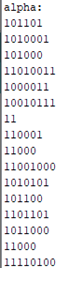
\includegraphics{alpha.png}
\caption{認証の際の$\alpha$}
\label{fig:alpha}
\end{minipage}
\begin{minipage}{0.33\hsize}
\centering
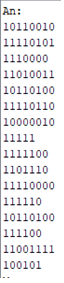
\includegraphics{beta_An.png}
\caption{認証情報$A_n$}
\label{fig:beta_An}
\end{minipage}
\begin{minipage}{0.33\hsize}
\centering
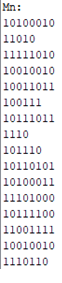
\includegraphics{beta_Mn.png}
\caption{秘匿情報$M_n$}
\label{fig:beta_Mn}
\end{minipage}
\end{figure}

\begin{figure}[H]
\begin{minipage}{0.33\hsize}
\centering
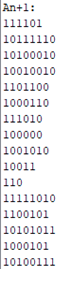
\includegraphics{beta_Am.png}
\caption{認証情報$A_{n+1}$}
\label{fig:beta_Am}
\end{minipage}
\begin{minipage}{0.33\hsize}
\centering
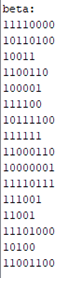
\includegraphics{beta.png}
\caption{$\beta$}
\label{fig:beta}
\end{minipage}
\begin{minipage}{0.33\hsize}
\centering
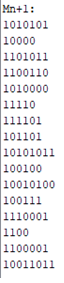
\includegraphics{ninsyo_Mm.png}
\caption{秘匿情報$M_{n+1}$}
\label{fig:ninsyo_Mm}
\end{minipage}
\end{figure}


暗号化の際に生成する$\gamma$の演算は$\gamma \leftarrow SD \oplus A_{n+1} \oplus A_n$である.
$\gamma \leftarrow SD \oplus A_{n+1} \oplus A_n$の演算は,シリアルモニタに表示させたビット列である図\ref{fig:SD}と図\ref{fig:beta_Am},図\ref{fig:beta_An}の3つの排他的論理和を演算し,その演算結果が図\ref{fig:gamma}になったことから,正しく演算されたと分かる.\\
暗号化の際に生成する認証情報の演算は$A_{n+2} \leftarrow \alpha \oplus A_{n+1} \oplus M_{n+1}$であり,$A_{n+2} \leftarrow \alpha \oplus A_{n+1} \oplus M_{n+1}$の演算は,シリアルモニタに表示させたビット列である図\ref{fig:ango_alpha}と図\ref{fig:beta_Am},図\ref{fig:ninsyo_Mm}の3つの排他的論理和の結果が図\ref{fig:ango_Al}になったことから,正しく演算されたと分かる.\\
暗号化の際に生成する次回秘匿情報の演算は$M_{n+2} \leftarrow A_{n+1} + M_{n+1}$であり,シリアルモニタに表示させたビット列である図\ref{fig:beta_Am}と図\ref{fig:ninsyo_Mm}の算術加算の結果が図\ref{fig:ango_Mm}になったことから,正しく演算されたと分かる.図\ref{fig:ango_Mm}では,$M_{n+1} \leftarrow M_{n+2}$で秘匿情報$M_{n+1}$に更新しているため,演算結果は$M_{n+1}$としてモニタに表示されている.\\

\begin{figure}[H]
\begin{minipage}{0.5\hsize}
\centering
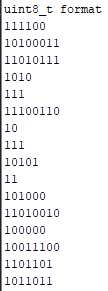
\includegraphics{SD.png}
\caption{$SD$}
\label{fig:SD}
\end{minipage}
\begin{minipage}{0.5\hsize}
\centering
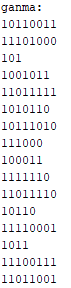
\includegraphics{gamma.png}
\caption{$\gamma$}
\label{fig:gamma}
\end{minipage}
\end{figure}

\begin{figure}[H]
\begin{minipage}{0.33\hsize}
\centering
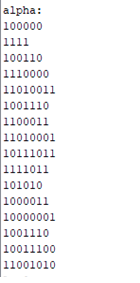
\includegraphics{ango_alpha.png}
\caption{暗号化通信の際の$\alpha$}
\label{fig:ango_alpha}
\end{minipage}
\begin{minipage}{0.33\hsize}
\centering
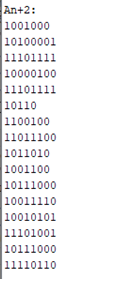
\includegraphics{ango_Al.png}
\caption{認証情報$A_{n+2}$}
\label{fig:ango_Al}
\end{minipage}
\begin{minipage}{0.33\hsize}
\centering
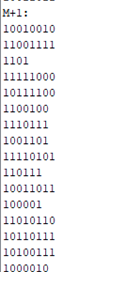
\includegraphics{ango_Mm.png}
\caption{秘匿情報$M_{n+2}$}
\label{fig:ango_Mm}
\end{minipage}
\end{figure}

\subsection{結合テスト}
結合テストでは基本設計を参考してテストを行った.結合テスト項目と結果を表\ref{tab:ketugo_test}に示す.
Arduinoはユーザー,Raspberry Piはサーバーと定義する.
\begin{table}[H]
\centering
\caption{結合テスト}
\label{tab:ketugo_test}
\scalebox{0.8}{
\begin{tabular}{|c|l|c|c|c|c|} \hline
 機能枠&確認内容&結果&確認日&確認者&備考欄\\ \hline\hline
 \multirow{5}{*}{認証} &
   認証要請の送受信を行う. &
   $\bigcirc$ & 2022/1/14 &
   \shortstack[l]{
   浅野\\
   内山田}&\\ \cline{2-6}
 & \shortstack[l]{
   認証の際,$\alpha$の送受信を行い,サーバーが送信\\
   したデータと,ユーザーが受信したデータ\\
   が一致している.} &
   $\bigcirc$ & 2022/1/14 &
   \shortstack[l]{
   浅野\\
   内山田}&
   \shortstack[l]{
   図\ref{fig:ninsyo_server_alpha}\\
   図\ref{fig:ninsyo_uv_alpha}}\\ \cline{2-6}
 & \shortstack[l]{
   認証の際,$\beta$の送受信を行い,ユーザーが送信\\
   したデータと,サーバーが受信したデータ\\
   が一致している.} &
   $\bigcirc$ & 2022/1/14 &
   \shortstack[l]{
   浅野\\
   内山田} &
   \shortstack[l]{
   図\ref{fig:ninsyo_uv_beta}\\
   図\ref{fig:ninsyo_server_beta}}\\ \cline{2-6}
 & 認証結果の送受信を行う. &
   $\bigcirc$ & 2022/1/14 &
   \shortstack[l]{
   浅野\\
   内山田}&\\ \cline{2-6}
 & \shortstack[l]{
   ユーザーで演算した\\
   認証情報$A_{n+1}$,秘匿情報$M_{n+1}$と,\\
   サーバーで演算した\\
   認証情報$A_{n+1}$,秘匿情報$M_{n+1}$が\\
   一致している.} &
   $\bigcirc$ & 2022/1/14 &
   \shortstack[l]{
   浅野\\
   内山田}&\\ \hline
\multirow{4}{*}{暗号化通信} & 
 \shortstack[l]{
   $\gamma$の送受信を行い,ユーザーが送信したデー\\
   タと,サーバーが受信したデータが一致し\\
   ている.} &
   $\bigcirc$ & 2022/1/14 &
   \shortstack[l]{
   浅野\\
   内山田}&
 \shortstack[l]{
   図\ref{fig:ninsyo_uv_gamma}\\
   図\ref{fig:ninsyo_server_gamma}}\\ \cline{2-6}
 & \shortstack[l]{
   ユーザーが取得したセンシングデータと日\\
   時が,データベースに保存されたセンシング\\
   データと日時と一致している. } &
   $\bigcirc$ & 2022/1/14 &
   \shortstack[l]{
   浅野\\
   内山田}&
 \shortstack[l]{
   図\ref{fig:ango_uv_sd}\\
   図\ref{fig:ango_server_sd}}\\ \cline{2-6}
 & \shortstack[l]{
   暗号化通信の際,$\alpha$の送受信を行い,サーバ\\
   ーが送信したデータと,ユーザーが受信した\\
   データが一致している.} &
   $\bigcirc$ & 2022/1/14 &
   \shortstack[l]{
   浅野\\
   内山田}&
   \shortstack[l]{
   図\ref{fig:ango_server_alpha}\\
   図\ref{fig:ango_uv_alpha}}\\ \cline{2-6}
 & \shortstack[l]{
   暗号化通信終了後,ユーザーとサーバーがそ\\
   れぞれ演算を行った認証情報$A_n$と秘匿情報\\
   $M_n$が一致している.} &
   $\bigcirc$ & 2022/1/14 &
   \shortstack[l]{
   浅野\\
   内山田}&\\ \hline
 \end{tabular}
}
\end{table}



サーバーが送信した$\alpha$は図\ref{fig:ninsyo_server_alpha}であり,
ユーザーが受信した$\alpha$は図\ref{fig:ninsyo_uv_alpha}であることから,
$\alpha$の値が一致しており,送受信が正しく行われたことが分かる.
\begin{figure}[H]
\begin{center}
	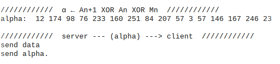
\includegraphics[width=10cm]{ninsyo_server_alpha.png}
	\caption{認証の際にサーバーが送信した$\alpha$}
	\label{fig:ninsyo_server_alpha}
\end{center}
\end{figure}
\begin{figure}[H]
\begin{center}
	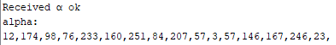
\includegraphics[width=10cm]{ninsyo_uv_alpha.png}
	\caption{認証の際にユーザーが受信した$\alpha$}
	\label{fig:ninsyo_uv_alpha}
\end{center}
\end{figure}

ユーザーが送信した$\beta$は図\ref{fig:ninsyo_uv_beta}であり,
ユーザーが受信した$\beta$は図\ref{fig:ninsyo_server_beta}であることから,
$\beta$の値が一致しており,送受信が正しく行われたことが分かる.

\begin{figure}[H]
\begin{center}
	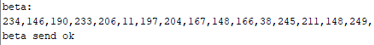
\includegraphics[width=10cm]{ninsyo_uv_beta.png}
	\caption{認証の際にユーザーが送信した$\beta$}
	\label{fig:ninsyo_uv_beta}
\end{center}
\end{figure}
\begin{figure}[H]
\begin{center}
	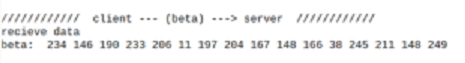
\includegraphics[width=10cm]{ninsyo_server_beta.png}
	\caption{認証の際にサーバーが受信した$\beta$}
	\label{fig:ninsyo_server_beta}
\end{center}
\end{figure}


ユーザーが送信した$\gamma$は図\ref{fig:ninsyo_uv_gamma}であり,
ユーザーが受信した$\gamma$は図\ref{fig:ninsyo_server_gamma}であることから,
$\gamma$の値が一致しており,送受信が正しく行われたことが分かる.

\begin{figure}[H]
\begin{center}
	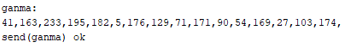
\includegraphics[width=10cm]{ninsyo_uv_gamma.png}
	\caption{暗号化通信の際にユーザーが送信した$\gamma$}
	\label{fig:ninsyo_uv_gamma}
\end{center}
\end{figure}
\begin{figure}[H]
\begin{center}
	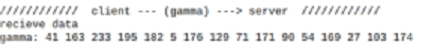
\includegraphics[width=10cm]{ninsyo_server_gamma.png}
	\caption{暗号化通信の際にサーバーが受信した$\gamma$}
	\label{fig:ninsyo_server_gamma}
\end{center}
\end{figure}

ある時点でユーザーが取得したセンシングデータと日時は図\ref{fig:ango_uv_sd}であり,
サーバーがデータベースに保存したセンシングデータと日時は図\ref{fig:ango_server_sd}
のデータベースに含まれていることから,センシングデータと日時が正しくデータベースに保存されたことが分かる.

\begin{figure}[H]
\begin{center}
	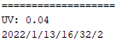
\includegraphics[width=4cm]{ango_uv_sd.png}
	\caption{ユーザーが取得したセンシングデータと日時}
	\label{fig:ango_uv_sd}
\end{center}
\end{figure}
\begin{figure}[H]
\begin{center}
	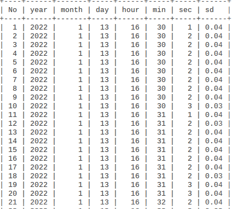
\includegraphics[width=10cm]{ango_server_sd.png}
	\caption{データベースに保存されたセンシングデータと日時}
	\label{fig:ango_server_sd}
\end{center}
\end{figure}

暗号化通信の際にサーバーが送信した$\alpha$は図\ref{fig:ango_server_alpha}であり,
ユーザーが受信した$\alpha$は図\ref{fig:ango_uv_alpha}であることから,
$\alpha$の値が一致しており,送受信が正しく行われたことが分かる.

\begin{figure}[H]
\begin{center}
	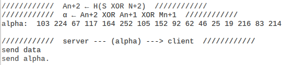
\includegraphics[width=10cm]{ango_server_alpha.png}
	\caption{暗号化通信の際にサーバーが送信した$\alpha$}
	\label{fig:ango_server_alpha}
\end{center}
\end{figure}
\begin{figure}[H]
\begin{center}
	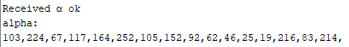
\includegraphics[width=10cm]{ango_uv_alpha.png}
	\caption{暗号化通信の際にユーザーが受信した$\alpha$}
	\label{fig:ango_uv_alpha}
\end{center}
\end{figure}

\subsection{総合テスト}
総合テストでは要件定義を参考してテストを行った.総合テスト項目と結果を表\ref{tab:sogo_test}に示す.
Arduinoはユーザー,Raspberry Piはサーバーと定義する.

\begin{table}[htbp]
\centering
\caption{総合テスト}
\label{tab:sogo_test}
\scalebox{0.7}{
\begin{tabular}{|c|l|c|c|c|c|} \hline
 機能枠&確認内容&結果&確認日&確認者&備考欄\\ \hline\hline
  \multirow{12}{*}{認証}
& ユーザーは起動後,1度時刻同期を行う.  &
   $\bigcirc$ & 2022/1/14 &
   \shortstack[l]{
   浅野\\
   内山田}&\\ \cline{2-6}
 & ユーザーが指定した時間に認証要請を送信する. &
   $\bigcirc$ & 2022/1/14 &
   \shortstack[l]{
   浅野\\
   内山田}&\\ \cline{2-6}
 & \shortstack[l]{
   複数のユーザーは同時刻に認証要請を送信するので,\\
   一台の認証が終了するまで,その他のユーザーは待機状態になる.} &
   $\bigcirc$ & 2022/1/14 &
   \shortstack[l]{
   浅野\\
   内山田}&\\ \cline{2-6}
 & ユーザーが認証処理を行っている. &
   $\bigcirc$ & 2022/1/14 &
   \shortstack[l]{
   浅野\\
   内山田}
& 図\ref{fig:sogo_ninsyo_uv}\\ \cline{2-6}
 & ユーザーが認証結果をモニタに表示している. &
   $\bigcirc$ & 2022/1/14 &
   \shortstack[l]{
   浅野\\
   内山田}&\\ \cline{2-6}
 & \shortstack[l]{ 
   認証が成功した場合,ユーザーがSAS-L2に基づいた\\
   暗号化通信を行う.} &
   $\bigcirc$ & 2022/1/14 &
   \shortstack[l]{
   浅野\\
   内山田}
 & \\ \cline{2-6}
 & \shortstack[l]{
   認証が失敗した場合,ユーザーはコネクションを切断して\\
  認証要請送信から再度開始する.} &
   $\bigcirc$ & 2022/1/14 &
   \shortstack[l]{
   浅野\\
   内山田}&\\ \cline{2-6}
 & サーバーが起動したら,受信待ち状態になる. &
   $\bigcirc$ & 2022/1/14 &
   \shortstack[l]{
   浅野\\
   内山田}&\\ \cline{2-6}
 & サーバーが認証要請受信後,認証処理を行っている. &
   $\bigcirc$ & 2022/1/14 &
   \shortstack[l]{
   浅野\\
   内山田}&
図\ref{fig:sogo_ninsyo_server_1}\\ \cline{2-6}
 & サーバーが認証結果をモニタに表示している. &
   $\bigcirc$ & 2022/1/14 &
   \shortstack[l]{
   浅野\\
   内山田}&\\ \cline{2-6} 
& \shortstack[l]{ 
   認証が成功した場合,サーバーがSAS-L2に基づいた暗号化通信を\\
   行う.} &
   $\bigcirc$ & 2022/1/14 &
   \shortstack[l]{
   浅野\\
   内山田}&\\ \cline{2-6}
 & \shortstack[l]{
   認証が失敗した場合,サーバーはコネクションを切断して\\
   認証要請の待ち状態となる.} &
   $\bigcirc$ & 2022/1/14 &
   \shortstack[l]{
   浅野\\
   内山田}&\\ \hline
 \multirow{9}{*}{暗号化通信}
 & ユーザーはセンシングデータを取得する. &
   $\bigcirc$ & 2022/1/14 &
   \shortstack[l]{
   浅野\\
   内山田}&\\ \cline{2-6}
 & \shortstack[l]{
   ユーザーは,シリアルモニタに取得したセンシングデータと\\
   センシングデータ取得日時を表示する.} &
   $\bigcirc$ & 2022/1/14 &
   \shortstack[l]{
   浅野\\
   内山田}
& \shortstack[l]{
図\ref{fig:pc_uv}\\
図\ref{fig:pc_mcp}\\
図\ref{fig:pc_hih}}\\ \cline{2-6}
 & \shortstack[l]{
   ユーザーはセンシングデータと日時を暗号化して\\
   サーバーへ送信する.} &
   $\bigcirc$ & 2022/1/14 &
   \shortstack[l]{
   浅野\\
   内山田}&\\ \cline{2-6}
 & ユーザーは暗号化通信を10回行う. &
   $\bigcirc$ & 2022/1/14 &
   \shortstack[l]{
   浅野\\
   内山田}&\\ \cline{2-6}
 & ユーザーは暗号化通信後,コネクションを切断する. &
   $\bigcirc$ & 2022/1/14 &
   \shortstack[l]{
   浅野\\
   内山田}&\\ \cline{2-6}
 & サーバーはセンシングデータと日時を復号する. &
   $\bigcirc$ & 2022/1/14 &
   \shortstack[l]{
   浅野\\
   内山田}&\\ \cline{2-6}
 & \shortstack[l]{
   サーバーはセンシングデータと取得日時を保存する際に,\\
   ユーザーごとのテーブルに分けて保存する.}  &
   $\bigcirc$ & 2022/1/14 &
   \shortstack[l]{
   浅野\\
   内山田}
 & \shortstack[l]{
図\ref{fig:db_uv}\\
図\ref{fig:db_hih}\\
図\ref{fig:db_mcp}}\\ \cline{2-6}
 & サーバーは暗号化通信を10回行う. &
   $\bigcirc$ & 2022/1/14 &
   \shortstack[l]{
   浅野\\
   内山田}&\\ \cline{2-6}
 &  \shortstack[l]{
   サーバーは暗号化通信後,コネクションを切断し\\
   認証要請待ち状態となる.} &
   $\bigcirc$ & 2022/1/14 &
   \shortstack[l]{
   浅野\\
   内山田}&\\ \hline
 \multirow{3}{*}{通信}
 & \shortstack[l]{
   ユーザーで,何らかのエラーが発生した場合,\\
   赤LEDを点滅させる.} &
   $\bigcirc$ & 2022/1/14 &
   \shortstack[l]{
   浅野\\
   内山田}&\\ \cline{2-6}
 & \shortstack[l]{
   サーバーは,5秒以上データを受信できなけ\\
   れば,コネクションを切断して認証要請\\
   受信の待機状態となる.} &
   $\bigcirc$ & 2022/1/14 &
   \shortstack[l]{
   浅野\\
   内山田}&\\ \cline{2-6}
& \shortstack[l]{
   3台のユーザーが同時刻に認証要請を送信した場合,\\
   3台のユーザーとの通信が10秒以内に完了する.}&
   $\bigcirc$ & 2022/1/14 &
   \shortstack[l]{
   浅野\\
   内山田}&\\ \hline
\end{tabular}
}
\end{table}
図\ref{fig:sogo_ninsyo_server_1}はサーバーのID:1のユーザーとの認証処理の結果であり,
図\ref{fig:sogo_ninsyo_uv}はID:1のユーザーの認証処理の結果をモニタに表示した図である.
サーバーは認証要請を受信後,生成した認証情報$A_{n+1}$を基に$\alpha$を生成し,ユーザーに送信している.
そして,サーバーはユーザーから$\beta$を受信し,認証結果をユーザーへ送信していると分かる.
ユーザーは認証要請を送信後,サーバーから受信した$\alpha$を基に$\beta$を生成し,サーバーに送信している.そして,ユーザーはサーバーから認証結果を受信し,認証結果から認証が成功したと分かる.
サーバーとID:2,ID:3の間での認証処理についても,同様に認証が成功したことを確認した.

\begin{figure}[H]
\begin{center}
	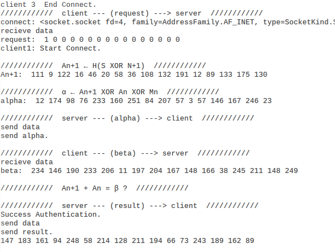
\includegraphics[width=10cm]{sogo_ninsyo_server_1.png}
	\caption{サーバーの認証結果}
	\label{fig:sogo_ninsyo_server_1}
\end{center}
\end{figure}
\begin{figure}[H]
\begin{center}
	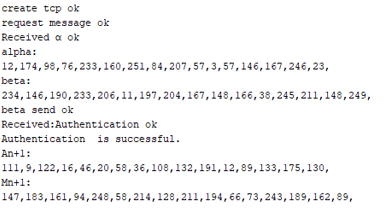
\includegraphics[width=10cm]{sogo_ninsyo_uv.png}
	\caption{ユーザーの認証結果}
	\label{fig:sogo_ninsyo_uv}
\end{center}
\end{figure}


ユーザーが取得したセンシングデータと日時は図\ref{fig:pc_uv}と図\ref{fig:pc_mcp},図\ref{fig:pc_hih}のようにシリアルモニタに表示されることが確認された.示した図はそれぞれある時点のものである.
サーバーがデータベースに保存したセンシングデータと日時は図\ref{fig:db_uv}と図\ref{fig:db_hih},
図\ref{fig:db_mcp}のようにユーザーのIDごとにテーブルに分て保存されていることが分かる.
また,ユーザーが取得したセンシングデータがデータベースに保存されていることから,ユーザーが取得したセンシングデータを暗号化してサーバーに送信し,サーバーがセンシングデータを復号できたことが分かる.

\begin{figure}[H]
\begin{center}
	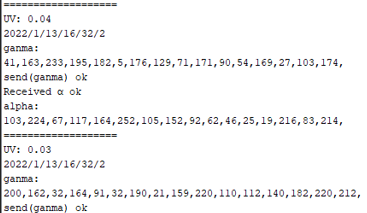
\includegraphics[width=10cm]{pc_uv.png}
	\caption{ID:1のシリアルモニタ}
	\label{fig:pc_uv}
\end{center}
\end{figure}
\begin{figure}[H]
\begin{center}
	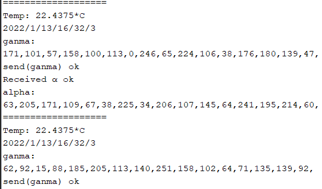
\includegraphics[width=10cm]{pc_mcp.png}
	\caption{ID:2のシリアルモニタ}
	\label{fig:pc_mcp}
\end{center}
\end{figure}
\begin{figure}[H]
\begin{center}
	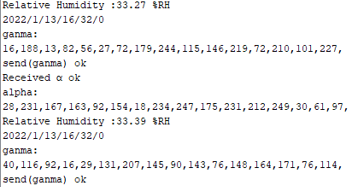
\includegraphics[width=10cm]{pc_hih.png}
	\caption{ID:3のシリアルモニタ}
	\label{fig:pc_hih}
\end{center}
\end{figure}

\begin{figure}[H]
\begin{center}
	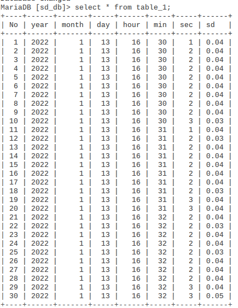
\includegraphics[width=10cm]{db_uv.png}
	\caption{データベースのID:1のテーブル}
	\label{fig:db_uv}
\end{center}
\end{figure}
\begin{figure}[H]
\begin{center}
	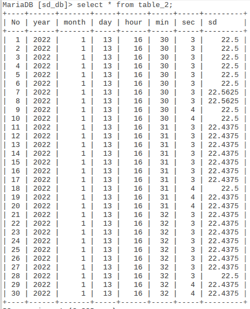
\includegraphics[width=10cm]{db_hih.png}
	\caption{データベースのID:2のテーブル}
	\label{fig:db_hih}
\end{center}
\end{figure}
\begin{figure}[H]
\begin{center}
	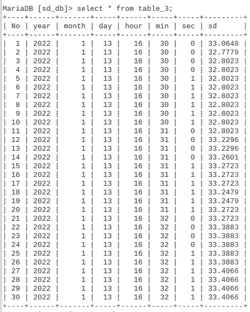
\includegraphics[width=10cm]{db_mcp.png}
	\caption{データベースのID:3のテーブル}
	\label{fig:db_mcp}
\end{center}
\end{figure}

\section{考察}
本節では,IoTにおけるセンシングデバイスでのセキュアなデータ通信の
実装での考察と問題点,今後の課題について述べる.

まず,本研究で開発したシステムの考察を述べる.
本研究では,SAS-L2認証方式をセンシングデバイスに実装することで,
デバイス間の認証とセンシングデータの暗号化通信方法の実現に成功した.
具体的に,認証については図\ref{fig:sogo_ninsyo_server_1}と図\ref{fig:sogo_ninsyo_uv}を用いて示したように,認証が成功したことからSAS-L2認証の実装が実現できたことが分かる.
そして,暗号化通信では,センシングデバイスが取得したセンシングデータを格納した$SD$と認証情報$A_n$と認証情報$A_{n+1}$の排他的論理和をサーバーへ送信し,サーバーがセンシングデータを復号してデータベースへ保存できたことからセンシングデバイスへの暗号化通信方法の実装が実現できたと分かる.

次に,本システムの問題点と今後の課題について述べる.
問題点の1つ目として,本研究ではセンシングデバイスがSAS-L2認証を用いてサーバーとのセキュアなデータ通信
を行うにあたり,初期認証情報と初期秘匿情報がセンシングデバイスに書き込まれていることが前提条件であることである.
実際では,センシングデバイスを生産するにあたり,初期情報が書き込まれているなら前提条件が満たされているが,
初期情報が書き込まれていないセンシングデバイスに関しては,安全な方法で初期情報を取得しなければならない.
安全な方法により初期情報を取得しなければ,悪意のある第三者により初期情報が盗聴され,
以後の認証・暗号化通信も盗聴・改ざんされる可能性がある.
初期情報が書き込まれていないセンシングデバイスである場合は,
初期情報を取得する安全な方法を確保しなければならないことが今後の課題である.


本研究ではエッジデバイスとしてArduino Leonardoを使用したが,Arduinoは電源を切った場合に初期化するため,
認証を行う度に認証情報と秘匿情報を不揮発性メモリに書き込まなければならない.
問題点の2つ目として,このようにセンシングデバイスが電源を切るたびに初期化してしまうものであった場合,
不揮発性メモリを使用しなくてはならないことである.不揮発性メモリは,デバイスの電源が切れても初期化されない
が,書き込み回数には限界がある.デバイスにより不揮発性メモリの寿命も様々であるが,認証回数が増える程に
メモリへの書き込み回数も増えるため,メモリの寿命が短くなる.
不揮発性メモリへの書き込みができなくなれば,認証・暗号化通信もできなくなるため,
一定時間内の認証の回数を決定する際,不揮発性メモリの書き込み回数の限界を考慮しなければならないことが課題である.



\chapter{あとがき}
%あとがき

本研究の研究背景としてIoTデバイスに対するセキュリティ対策として認証・暗号化通信を行うことが挙げられるが,処理性能の低いIoTデバイスでは従来法の暗号方式での実装が困難である.
そこで,本研究ではワンタイムパスワード認証方式SAS-L2をIoTセンシングデバイス
に実装することで,デバイス間の認証およびセンシングデータの暗号化通信方法を実現することを目標に開発を行った.
SAS-L2認証方式を導入したIoTシステムの設計はUMLのユースケース図,クラス図,シーケンス図などを用いて行い,
その設計に基づきチームで分担し開発を行った.実装完了後は,V字開発モデルに従って,単体テスト,結合テスト,総合テストの順でテストを行った.
検証結果から,SAS-L2認証方式をセンシングデバイスに実装し,
デバイス間の認証とSAS-L2に基づいたデータ通信の暗号化ができたことが分かる.
また,センシングデータの暗号化では,排他的論理演算2回で済むため,処理能力の低いセンシングデバイスにおいてリアルタイムでの暗号化通信を実現することができる.
そして,問題点と課題として,センシングデバイスに初期認証情報や初期秘匿情報が書き込まれていない場合,
初期情報を取得する際の安全な方法の確立について,そして,認証情報と秘匿情報を不揮発性メモリに書き込む場合,
不揮発性メモリの書き込み回数を考慮して認証回数の決定をしなくてはならないという点が挙げられる.
それらを改善することで,本システムでの処理性能の低いセンシングデバイスに認証方式と暗号化通信を導入することによる,さらなるセキュリティ強化に繋がると考える.


%謝辞
\newpage
\addcontentsline{toc}{chapter}{\protect\numberline{謝辞}{}}
\chapter*{謝辞}
%--ここから謝辞--

本研究を進めるにあたり,懇篤な御指導,御鞭撻を賜わりました本学高橋寛教授に深く御礼申し上げます.

本論文の作成に関し,詳細なるご検討,貴重な御教示を頂きました本学高橋寛教授ならびに甲斐博准教授,王森レイ講師に深く御礼申し上げます.

また,審査頂いた本学高橋寛教授,樋上喜信教授,井門俊講師に深く御礼申し上げます.

最後に,多大な御協力と貴重な御助言を頂いた本学工学部情報工学科情報システム工学講座高橋研究室の諸氏に厚く御礼申し上げます.

%--ここまで謝辞--

%参考文献
\begin{thebibliography}{99}
%ここから参考文献

\bibitem{maegaki}
IPA独立行政法人情報処理推進機構技術本部セキュリティセンター.“IPAテクニカルウォッチ「自動車の情報セキュリティ」に関するレポート".IPA独立行政法人情報処理推進機構.
\url{https://www.ipa.go.jp/files/000009384.pdf},
(参照2022-01-05)
\bibitem{AES}
斉藤貴之.“3分でわかるAES".日経クロステック.
\url{https://xtech.nikkei.com/atcl/nxt/keyword/18/00002/030800119/},
(参照2022-01-05)
\bibitem{banamu}
“最強の暗号?バーナム暗号".kakke18's blog.2019-02-22.
\url{https://kakke18.hatenablog.com/entry/2019/02/22/193223},
(参照2022-01-05)
\bibitem{tcp/udp}
竹下隆史,村山公保,荒井透,苅田幸雄.マスタリングTCP/IP入門編第5版.オーム社.2019.
\bibitem{sas-l}
清水明宏.SAS-L ワンタイムパスワード認証方式について.preprint.2020.
\bibitem{vmodel}
水野忠則,中篠直也,井上雅裕,山田圀裕.未来へつなぐデジタルシリーズ20 組込システム.共立出版.2017.
\bibitem{uml}
永和システムマネジメント.“UML超入門".オブラブ.
\url{http://objectclub.jp/technicaldoc/uml/umlintro},
(参照2022-01-05)
%ここまで参考文献

\end{thebibliography}
\end{document}



